\documentclass[11pt,a4paper]{article}
\usepackage[colorinlistoftodos]{todonotes}
% THE FIGURE NUMBERS GOT MIXED UP BECAUSE WE STARTED MOVING THEM AROUND

% Suggestions for Holger:
% 1) Error plots (Figures 10, 11): smooth high-frequency errors, plot 9 lines on one plot (1d,10d,30d) * (3 C pools) for each site. This will result in 3 plots (1 for each site)
% Holger:
%   --> Do you mean figures 8,9 (relative error)? YES
%   --> 360-day moving average could do the smoothing: SOUNDS GOOD
%   --> 3 color x 3 line types = 9 lines per plot
% Holger 2:
%   --> Why would we actually like to smooth the error. Isn't it nice to see a wild noise around zero?



% 2) Create relative error figure for 14C analogous to new figures from #10 and #11
% Holger:
%   --> again: figures 8, 9?: YES, ANALOGOUS TO 8,9
%   --> only 14C  or also Delta 14C?: I THINK 14C
% Holger 2:
%   --> done for 1d and 10d




% 3) Delete Figures 8 and 9 (absolute error), they are duplicative of Figures 10, 11
% Holger:
%   --> figures 6 and 7 show absolute error
% Holger 2:
%   --> deleted figures with absolute error, kept relative error figures




% 4) Delete figures 6 and 7
% Holger:
%   --> I guess you mean figures 4 and 5?:YES
% Holger 2:
%   --> deleted



% 5) Figures 12 and 13 consolidated to one figure with 30 d time step (we're assuming the error for 30 d is still very small. If it's less than 1-10 percent, it's probably fine)
% Holger:
%   --> Do you mean 10 and 11 here (depth profiles of Delta 14C)?: YES
% Holger 2:
%   --> deleted 1d figure, kept 10d figure



% 6) Figures 14 and 15: consolidate to a single figure, column integrated, with 30 d time step. Add atmosphere 14C content. Make clear the difference between ELM and reconstruction using solid and dashed lines
% Holger:
%   --> 12, 13?: YES
%   --> At the moment these figures are column integrated.
%   --> Solid and dashed lines can hardly emphasize a difference, because they lie on top of each other. That's why I used dots for the discrete reconstruction.: BUT THE DOTS ARE NOT CLEAR. BIGGER?
%% Holger 2:
%   --> deleted 1d figure, kept 10d figure, increased dot size, added atmosphere, unified axes scales
%   --> filename: Delta_14C_through_time_per_pool.pdf




% 7) Figures 16 and 17: (depth resolved) remove these figures
% Holger:
%   --> 14, 15?: YES
%% Holger 2:
%   --> done


%%%%% for debugging %%%%%

\usepackage{xcolor}
\newcommand{\red}[1]{\textcolor{red}{#1}}
\newcommand{\blue}[1]{\textcolor{blue}{#1}}
\newcommand{\gray}[1]{\textcolor{gray}{#1}}

%%%%% true header %%%%%

\usepackage{authblk}
\usepackage{natbib}
\usepackage{graphicx}
\usepackage{booktabs}
\usepackage{amsmath,amssymb,amsfonts,amscd,amsthm}
\usepackage{bm}
\usepackage{pdflscape}
\usepackage[flushleft]{threeparttable}
\usepackage{lineno}
\usepackage{setspace}
\usepackage{textcomp}
\usepackage{times}
\usepackage{enumerate}
\usepackage{rotating}

%%%%% units %%%%%
\usepackage{siunitx}
\sisetup{output-exponent-marker=\ensuremath{\mathrm{e}}}
\DeclareSIUnit\yr{yr}

%%%%% personal definitions %%%%
% vectors and matrices
\renewcommand{\vec}[1]{\mathbf{#1}}
\newcommand{\tens}[1]{\mathrm{#1}}
\newcommand{\id}{\tens{Id}}

% integrals
\newcommand{\deriv}[1]{\frac{\mathrm{d}}{\mathrm{d}#1}}
\newcommand{\dd}[1]{\,\mathrm{d}#1}

% limits and sums
\newcommand{\intl}{\int\limits}
\newcommand{\suml}{\sum\limits}

% spaces
\newcommand{\R}{\mathbb{R}}

%%%%% title page data %%%%%

%\title{\bf Inferring radiocarbon values in carbon cycle models from their numerical output}
\title{\bf Model reconstruction and computation of soil radiocarbon from the numerical output of land carbon models}
\author[1]{Holger Metzler}
\author[2]{William Riley}
\author[2]{Qing Zhu}
\author[1]{Alison Hoyt}
\author[1]{Markus M\"uller}
\author[1]{Carlos A. Sierra}
\affil[1]{\it \small Max Planck Institute for Biogeochemistry, Hans-Kn\"oll-Str. 10, 07745 Jena, Germany}
\affil[2]{\it Climate and Ecosystem Sciences Division, Lawrence Berkeley National Laboratory, Berkeley 94720, USA}

\date{}

\begin{document}
\doublespace
\maketitle

\noindent
{\bf Running head}: Radiocarbon from model output

\vspace{2em}

\noindent
\textbf{Corresponding author}: \\ Carlos A. Sierra, Max-Planck-Institute for Biogeochemistry, Hans-Kn\"{o}ll-Str. 10, 07745 Jena, Germany. Phone: +49 3641 576133, fax: +49 3641 577100, email: csierra@bgc-jena.mpg.de.

\vspace{2em}

\noindent
{\bf Keywords}: carbon cycle models, carbon stocks, carbon fluxes, reservoir theory, compartment models, radiocarbon, dynamical systems,  model diagnostics

\vspace{2em}

\noindent
{\bf Type of paper}: Technical Advance; possible journals: GCB, JAMES, GMD
\newpage
\linenumbers

\begin{abstract}
Radiocarbon is a powerful tracer of the global carbon cycle that is commonly used to assess rates of carbon cycling in different Earth system reservoirs, and as benchmark to assess model performance. It is increasingly recognized that radiocarbon should be included in Earth system models, and it has been recommended that models for the sixth model inter-comparison project CMIP6 report the predicted radiocarbon values for a multitude of carbon pools. However, the inclusion of radiocarbon in many models puts an additional burden on model developers that may not have the time or resources for a detailed representation of radiocarbon dynamics. Here, we present an alternative approach that \red{consists on} computing radiocarbon values for carbon pools from the numerical output of the model. It requires the use of the computed stocks and fluxes among all carbon pools for a particular simulation of the model. From this output, it is possible to compute a time-dependent linear compartmental system with its respective state transition matrix. \todo[color=green!40]{matrix or operator?} Using reported values of atmospheric radiocarbon as inputs to the system, the state transition matrix is then applied to compute radiocarbon values for each individual pool, the average value for the entire system, and the radiocarbon in the output flux. 
%These quantities are compared with pool ages, system ages, and transit times of carbon for the particular simulation being analyzed. 
We demonstrate the approach for the soil component of ELMv1-ECA, a vertically resolved model that already explicitly includes radiocarbon and includes seven pools and ten vertical layers. Results from our proposed method are nearly identical to the predictions of ELMv1-ECA, which shows the great potential for using this approach in not only CMIP6 models that do not include radiocarbon, but also model output from previous model inter-comparison exercises. \todo[color=green!40]{strange last sentence}
\end{abstract}

\newpage

\section{Introduction}
%\begin{itemize}
%\item Radiocarbon as a tracer of the global carbon cycle
%\item Recommendation to include radiocarbon in CMIP6 models
%\item \gray{Introduce approach developed by Metzler et al. to compute age and transit times in time-dependent nonlinear models}
%\item Introduce aims of the paper and organization
%\end{itemize}

Terrestrial ecosystems, and soils in particular, are an important global C reservoir but with large uncertainties in the controls on soil C cycling, and its representation in models \citep{Luo2016}. The dynamics of radiocarbon in terrestrial ecosystems can be used to interpret the rates at which carbon is exchanged with the atmosphere and moves through vegetation and soils. As a result, radiocarbon has been used in many empirical studies to evaluate rates of soil C cycling. However, it has only more recently been used as a tool for model intercomparison \citep{He2016}. 

Measurements of radiocarbon offer great potential to constrain temporal dynamics of ecosystem models and to assess their performance. However, to date, such comparisons have been limited to a small number of models which simulate C isotopes \citep[e.g.][]{Koven2013, Tifafi2018}, as the majority of models do not explicitly represent isotope dynamics. The current coupled climate-carbon cycle model intercomparison project (C4MIP) of the 6th phase coupled model intercomparison project (CMIP6), requests model participants to explicitly model radiocarbon and include the corresponding output from the major land and ocean model compartments \citep{Jones2016}. \todo[color=green!40]{repetition}However, to date, many models do not represent radiocarbon, as it can be time-consuming to implement, and computationally intensive to run. Thus, the goal of this work is to develop a tool to make radiocarbon-based comparisons of C cycling comparable across a wider suite of models.

The availability of radiocarbon output from a range of models would allow not only an additional data constraint against global datasets \citep{He2016, Mathieu2015}, it may also offer a new tool for differentiating patterns of C cycling across different model structures \citep{Sierra2014}. 
%There are two broad classes of models currently being applied for studies of the global carbon cycle: (1) pseudo-first order representations, based on concepts first described for Century (Parton et al. 1996) and RoTHC (cite) and (2) microbe and mineral-surface explicity models (eg Ahrens et al. 20XX, Dwivedi et al. 2017; Riley et al. 2014; Sulman et al 2018) that attempt to more explicitly represent the underlying mechanisms responsible for soil carbon transformations. 
% I removed this sentence because the classification portrayed here is too simple. 
There are literally hundreds of different models of soil carbon cycling proposed in the literature \citep{Manzoni2009SBB}, each portraying different hypotheses about internal system dynamics, with specific model structures and parameterizations. Broad generalizations of models have been proposed based on basic assumptions of soil organic matter dynamics \citep{Sierra2015}.
Computing radiocarbon output from these different classes of models, without the need to incorporate isotopes into the full model structure, would allow more widespread data-model comparison, and an enhanced ability to evaluate differences in the way soil C cycles in these models.

Linear response theory suggests that the impulse response function of a particular model can be used to compute isotope dynamics without explicitly simulating the isotope within the model, but rather using the response function to convolve the isotope tracer \citep{Thompson1999}. This means that it may not be necessary to explicitly represent isotope dynamics a priori in a model, but it can be obtained a posteriori through the convolution procedure. However, linear response theory relies on assumptions of linearity and steady-state of the model, which are not met for the type of transient simulations to be submitted to C4MIP. 

\citet{Metzler2018PNAS} recently developed a method to obtain a mathematical object, the state transition matrix (see details below), that generalizes response function theory for nonlinear models out of equilibrium. This approach removes previous assumptions that prevented the use of the linear response approach for the computation of isotope and tracer dynamics a posteriori from simulations. Therefore, it offers an opportunity to compute isotope dynamics from models that do not explicitly represent it, and could be applied to models from CMIP6. Since output from these MIPs is presented in discrete time steps, it is still a challenge to translate the state transition matrix approach from the continuous to the discrete case.

We present an approach to compute radiocarbon values for models which do not explicitly represent it. To this end, we extend the approach presented in \citet{Metzler2018PNAS} for the computation of the state transition matrix in continuous time to the discrete time case, and apply it to reconstruct tracer and isotope dynamics from model output. We first give a mathematical overview of the approach and then present examples of its use. We test our approach by comparing our computed values to output from the ELMv1-ECA model, an Earth system model that explicitly represents radiocarbon. We successfully match the modeled radiocarbon values along the entire vertically resolved soil profile, across soil and litter pools over time. This is a valuable new framework with large potential for application to the CMIP archives and to models with more diverse structures. 

\section{Methods}
\subsection{Carbon cycle models as compartmental systems}
    Carbon cycle models are subject to the law of mass conservation and therefore can be represented as compartmental systems \citep{Anderson1983, Jacquez1993}.
    A compartmental system with $d\geq1$ compartments is of the general form of the initial value problem
    \begin{equation}\label{eqn:CS_td_nonlin}
        \begin{aligned}
            \deriv{t}\,\vec{C}(t) &= \tens{B}(\vec{C}(t),t)\,\vec{C}(t) + \vec{u}(\vec{C}(t),t),\quad t>t_0,\\
            \vec{C}(t_0) &= \vec{C}^0.
        \end{aligned}
    \end{equation}
    Here, $\vec{C}(t)$ is the vector of compartment contents at time $t$, $\tens{B}$ is a matrix-valued function that governs the cycling of carbon through the system, $\vec{u}(t)$ is the vector of external carbon inputs to the system, $t_0$ is some fixed initial time, and $\vec{C}^0$ is a given vector  of initial system contents. Note that the internal cycling as well as the external inputs can each depend on time (e.g. due to changing environmental conditions) and on the current carbon content of the system itself. Consequently, system \eqref{eqn:CS_td_nonlin} is time-dependent and nonlinear.
    
    To guarantee mass conservation, the matrix $\tens{B}(\vec{x},t)$ is required to be compartmental 
    %\todo{can we clarify what 'compartmental' means? above you say mass conservation defines being compartmental, so this sentence seems tautological?} \todo[color=green!40]{the definition of the matrix being compartmental is the following list of (i), (ii), (iii)} 
    for all nonnegative $\vec{x}$ and $t>t_0$, i.e., $\tens{B}(\vec{x},t)=(\tens{B}_{ij}(\vec{x},t))_{i,j=1,2,\ldots,d}$ satisfies the properties
    \begin{enumerate}[(i)]
        \item $B_{ii}(\vec{x},t)\leq0$ for all $i$,
        \item $B_{ij}(\vec{x},t)\geq0$ for all $i\neq j$,
        \item $\suml_{i=1}^d B_{ij}(\vec{x},t)\leq0$ for all $j$.
    \end{enumerate}
    The diagonal values of $B_{ii}$ can be interpreted as the cycling rate of compartment $i$, the off-diagonal entries $B_{ij}$ represent the rate of carbon flux from compartment $j$ to compartment $i$, and $z_j=-\sum_{i=1}^d B_{ij}$ is the rate of carbon leaving the system through pool $j$.
    
    We now assume that we know a unique (numerical) solution $\vec{C}=\vec{C}(t)$ of system \eqref{eqn:CS_td_nonlin}.
    Plugging this solution into the system, we obtain a new compartmental system
    \begin{equation}\label{eqn:CS_td_lin}
        \begin{aligned}
            \deriv{t}\,\widetilde{\vec{C}}(t) &= \widetilde{\tens{B}}(t)\,\widetilde{\vec{C}}(t) + \widetilde{\vec{u}}(t),\quad t>t_0,\\
            \widetilde{\vec{C}}(t_0) &= \vec{C}^0,
        \end{aligned}
    \end{equation}
    where $\widetilde{\tens{B}}(t)=\tens{B}(\vec{C}(t),t)$ and $\widetilde{\vec{u}}(t)=\vec{u}(\vec{C}(t),t)$.
    This system is still time-dependent, but not nonlinear anymore.
    Under the assumption that it has a unique solution $\widetilde{\vec{C}}=\widetilde{\vec{C}}(t)$, the two solution trajectories $\widetilde{\vec{C}}$ and $\vec{C}$ are identical.
    Then the linear compartmental system \eqref{eqn:CS_td_lin} describes exactly the same solution trajectory as the nonlinear compartmental system \eqref{eqn:CS_td_nonlin}.
    For the sake of simplicity of notation we omit the tilde in Eq. \eqref{eqn:CS_td_lin} from now on.
    
    The unique semi-analytical solution of linear compartmental system \eqref{eqn:CS_td_lin} is given by \citep{Brockett2015}
    \begin{equation*}
        \vec{C}(t) = \tens{\Phi}(t,t_0)\,\vec{C}^0 + \intl_{t_0}^t \tens{\Phi}(t,\tau)\,\vec{u}(\tau)\dd{\tau}.
    \end{equation*}
    We call the solution semi-analytic because the system's state transition matrix $\tens{\Phi}$ is only implicitly given as the unique solution of the matrix initial value problem
    \begin{equation*}
        \begin{aligned}
            \deriv{t}\,\tens{\Phi}(t,t_0) &= \tens{B}(t)\,\tens{\Phi}(t,t_0),\quad t>t_0,\\
            \tens{\Phi}(t_0,t_0) &= \id,
        \end{aligned}
    \end{equation*}
    where $\id$ denotes the identity matrix in $\R^d$. 
%    \todo{then why not just use that symbol?} \todo[color=green!40]{$\R^d$ is the $d$-dimensional space on which the identity matrix $\id$ acts., i.e. $\id:\R^d\to\R^d$ by $\id x=x$ for $x\in\R^d$.}

    %\red{Bill: what about vertical structure and transport? Shouldn't we introduce that here also?}
    %\todo[inline, color=green!40]{I will introduce here more explicitly how to do that}
    
    \subsubsection*{Representation of depth-resolved systems}
    This framework also incorporates also depth-resolved systems.
    Think of a depth-resolved compartmental model with $l$ depth layers and $c$ compartment types per layer.
    Let $d:=c\,l$.
    The numbers $1,2,\ldots,l$ belong to layer $1$, layer $2$,\,\ldots,\,layer $l$ of compartment type $1$, respectively.
    The numbers $l+1,l+2,\ldots,2\,l$ belong to layer $1$ through layer $l$ of compartment type $2$; and so forth.
    Eventually, the numbers $(c-1)\,l+1,(c-1)\,l+2,\ldots,c\,l$ belong to layers $1$ through $l$ of compartment type $c$.
    We introduce $\tens{B}:=(B_{ij})_{i,j=1,2,\ldots,d}$ and $\vec{u}:=(u_i)_{i=1,2,\ldots,d}$.
    Then the depth-resolved system fits in the framework of Eq. \eqref{eqn:CS_td_nonlin}.
    For a system with $l=10$ depth layers and $c=7$ compartment types per layer, $\tens{B}$ is a $70\times 70$-matrix, and $\vec{u}$ is a vector with $70$ components.
    For example, $B_{12,11}$ is the flux rate downwards from layer $1$ to layer $2$ of compartment type $1$, and $B_{35,55}$ is the flux rate from compartment type $5$ to compartment type $3$ within depth layer number $5$ (recall that the first index represents the target and the second index the source).
    Note that also vertical fluxes between different compartment types can be represented, e.g. by $B_{23,52}$.
    The negative diagonal entries $(B_{ii})_{i=1,2,\ldots,70}$ are the total exit rates of the compartments, i.e. the rates to other compartment types in any layer plus the rate of material leaving from the system.
    

\subsection{The radiocarbon compartmental system}
    Once we know the representation \eqref{eqn:CS_td_nonlin} of a carbon cycle model, we can readily manipulate the equation to obtain a compartmental system for radiocarbon.
    We only need to substitute $\tens{B}$ by ${}^{14}\tens{B}$ defined by
    \begin{equation*}
        {}^{14}\tens{B}(\vec{C}(t),t) = \tens{B}(\vec{C}(t),t) - \lambda\,\id,
    \end{equation*}
    where $\lambda$ is the radioactive decay constant of ${}^{14}$C scaled to the right time unit.
    For example, if the system is observed in time units of years, then $\lambda=\ln(2)/5568$.
    This manipulation leads to a state transition matrix of the radiocarbon system given by
    \begin{equation*}
        {}^{14}\tens{\Phi}(t,t_0) = \tens{\Phi}(t,t_0)\, e^{-\lambda\,(t-t_0)}\,\id, \quad t\geq t_0,
    \end{equation*}
    from which we can directly see the effect of the radioactive decay.


%\section{Approach to reconstruct a carbon cycle model from data}
\subsection{Reconstruction of a continuous-time system from discrete-time model output}
The approach presented above works only when we have the original model completely described by a system of ODEs, which by definition implies that the system is continuous in time. However, we are interested in using the approach for ESMs for which we only have access to model output reported in discrete time steps. Therefore, it is necessary to reconstruct a Continuous-Time Approximation (CTA) model from this discretm oedel output. 
    
    \subsubsection*{One compartment case}
        Suppose we are given a one compartment time-dependent linear compartmental system
        \begin{equation}\label{eqn:CS_one_dim}
            \begin{aligned}
                \deriv{t}\,C(t) &= \gamma(t)\,C(t) + u(t),\quad t>t_0,\\
                C(t_0) &= C^0,
            \end{aligned}
        \end{equation}
        of which $\gamma(t)$ and $u(t)$ are unknown.
        But for discrete times $t_0<t_1<t_2<\cdots<t_n$ we are given
        \begin{itemize}
            \item the initial system content $C^0$,
            \item $u^k = \intl_{t_k}^{t_{k+1}} u(t)\dd{t},\quad k=0,1,\ldots,n-1$, and
            \item $r^k = \intl_{t_k}^{t_{k+1}} r(t)\dd{t},\quad k=0,1,\ldots,n-1$.
        \end{itemize}
        Here, $u^k$ and $r^k$ denote the accumulated external system input and the accumulated external system output in the time interval $I_k=[t_k,t_{k+1}]$, $k=0,1,\ldots,n-1$, respectively.

        We are interested in constructing a compartmental system, as simple as possible, that matches these given data as well as possible.
        To that end, we approximate the (unknown) system \eqref{eqn:CS_one_dim} on each interval $I_k$ by a linear time-independent system
        \begin{equation}\label{eqn:CS_one_dim_approx}
            \begin{aligned}
                \deriv{t}\,\widehat{C}(t) &= \widehat{\gamma}^k\,\widehat{C}(t) + \widehat{u}^k,\quad t\in I_k,\\
                \widehat{C}(t_k) &= \widehat{C}^k.
            \end{aligned}
        \end{equation}
        Suppose that at time step $k$ the value $\widehat{C}^k$ is already known from the previous time step,
        and for $k=0$ we set $\widehat{C}^0=C^0$.
        
        We write $\Delta_k=t_{k+1}-t_k$ and choose $\widehat{u}^k=u^k/\Delta_k$.
        Consequently, for the time interval $I_k$ the cumulative external system input $u^k$ of the unknown system \eqref{eqn:CS_one_dim} and the cumulative external system input $\Delta_k\,\widehat{u}^k$ of the approximating system \eqref{eqn:CS_one_dim_approx} coincide.
        We are left with finding good approximations $\widehat{\gamma}^k$ for $\gamma(t)$ on $I_k$, $k=0,1,\ldots,n-1$.
        We can compute the cumulative external system output of the approximating system \eqref{eqn:CS_one_dim_approx} on $I_k$, in dependence on the choice of $\widehat{\gamma}^k$, by
        \begin{equation*}
            \widehat{r}^k(\widehat{\gamma}^k) = -\widehat{\gamma}^k\intl_{t_k}^{t_{k+1}} \widehat{C}(t)\dd{t},
        \end{equation*}
        where, for $t\in I_k$,
        \begin{align*}
            \widehat{C}(t) &= e^{-\widehat{\gamma}^k\,(t-t_k)}\,\widehat{C}^k + \intl_{t_k}^t e^{-\widehat{\gamma}^k\,(t-\tau)}\,\widehat{u}^k\dd{\tau}\\
            &= e^{-\widehat{\gamma}^k\,(t-t_k)}\,\widehat{C}^k + (\widehat{\gamma}^k)^{-1}\,(e^{-\widehat{\gamma}^k\,(t-t_k)}-1)\,\widehat{u}^k
        \end{align*}
        is the unique solution of \eqref{eqn:CS_one_dim_approx} on $I_k$.
        Consequently, we obtain $\widehat{\gamma}^k$ by solving the one-dimensional nonlinear optimization problem
        \begin{equation*}
            \underset{\widehat{\gamma}^k<0}{\operatorname{minimize}}\,|\widehat{r}^k(\widehat{\gamma}^k)-r^k|.
        \end{equation*}
        We define $\widehat{C}^{k+1}=\widehat{C}(t_{k+1})$ and continue with the next time step $k+1$.
        
        In the special case of a time-independent unknown system \eqref{eqn:CS_one_dim}, i.e. $\gamma(t)=\gamma<0$ and $u(t)=u\geq0$, the approximation by system \eqref{eqn:CS_one_dim_approx} is perfect, independent of the number $n$ of given data points.\\
        
    \subsubsection*{Mutli compartment case}
        If the compartmental system consists of more than one compartment, internal cycling among the different compartments may occur. As described below, all modern soil carbon models are multi-compartmental, and they often represent vertical structure with explicit representation of diffusive or advective fluxes that connect adjacent soil layers in the discretized model.
        An approximating system is then required to also match the internal fluxes.
        Suppose we are given a $d$-compartment time-dependent linear system
%        \begin{equation}\label{eqn:CS_two_dim}
%            \begin{aligned}
%                \deriv{t}\,\begin{pmatrix} C_1 \\ C_2 \end{pmatrix}(t) &= 
%                \begin{pmatrix} B_{11} & B_{12} \\ B_{21} & B_{22} \end{pmatrix}(t)\,
%                \begin{pmatrix} C_1 \\ C_2 \end{pmatrix}(t) + 
%                \begin{pmatrix} u_1 \\ u_2 \end{pmatrix}(t),\quad t>t_0,\\
%                \begin{pmatrix} C_1 \\ C_2 \end{pmatrix}(t_0) &=
%                \begin{pmatrix} C^0_1 \\ C^0_2 \end{pmatrix},
%            \end{aligned}
%        \end{equation}
        \begin{equation}\label{eqn:CS_multi_dim}
            \begin{aligned}
                \deriv{t}\,\vec{C}(t) &= \tens{B}(t)\,\vec{C}(t) + \vec{u}(t),\quad t>t_0,\\
                \vec{C}(t_0) &= \vec{C}^0,
            \end{aligned}
        \end{equation}
        of which $\tens{B}(t)=(B_{ij}(t))_{i,j=1,2,\ldots,d}$ and $\vec{u}(t)=(u_i(t))_{i=1,2,\ldots,d}$ are unknown.
        But for discrete times $t_0<t_1<t_2<\cdots<t_n$ we are given
        \begin{itemize}
            \item the initial system content vector $\vec{C}^0=(C^0_1,C^0_2,\ldots,C^0_d)^T$,
            \item $\vec{u}^k = \intl_{t_k}^{t_{k+1}} \vec{u}(t)\dd{t},\quad k=0,1,\ldots,n-1$, 
            \item $\vec{r}^k = \intl_{t_k}^{t_{k+1}} \vec{r}(t)\dd{t},\quad k=0,1,\ldots,n-1$, and
            \item $F_{ij}^k = \intl_{t_k}^{t_{k+1}} B_{ij}(t)\,C_j(t)\dd{t},\quad i\neq j$.
        \end{itemize}
        Here, $\vec{u}^k$ and $\vec{r}^k$ denote the accumulated external system input vector and the accumulated external system output vector in the time interval $I_k=[t_k,t_{k+1}]$, $k=0,1,\ldots,n-1$, respectively.
        Furthermore, $F^k_{ij}$ denotes the accumulated flux from compartment $j$ to compartment $i$ during $I_k$.

        We are interested in constructing a compartmental system, as simple as possible, that matches these given data as well as possible.
        To that end, we approximate the (unknown) system \eqref{eqn:CS_multi_dim} on each interval $I_k$ by a linear time-independent system
        %\todo{Why do you call this time-independent, when time is in the equation?} \todo[color=green!40]{because $\tens{B}$ and $\vec{u}$ do not depend on time $t$, then this is the usual terminology: time-independent or autonomous}
        \begin{equation}\label{eqn:CS_multi_dim_approx}
            \begin{aligned}
                \deriv{t}\,\widehat{C}(t) &= \widehat{\tens{B}}^k\,\widehat{C}(t) + \widehat{\vec{u}}^k,\quad t\in I_k,\\
                \widehat{\vec{C}}(t_k) &= \widehat{\vec{C}}^k.
            \end{aligned}
        \end{equation}
        Suppose that at time step $k$ the vector $\widehat{\vec{C}}^k$ is already known from the previous time step.
        This is no restriction, because for $k=0$ we set $\widehat{\vec{C}}^0=\vec{C}^0$.

        Again, we write $\Delta_k=t_{k+1}-t_k$ and choose $\widehat{\vec{u}}^k=\vec{u}^k/\Delta_k$.
        Consequently, for the time interval $I_k$ the cumulative external system input vector $\vec{u}^k$ of the unknown system \eqref{eqn:CS_multi_dim} and the cumulative external system input vector $\Delta_k\,\widehat{\vec{u}}^k$ of the approximating system \eqref{eqn:CS_multi_dim_approx} coincide.
        We are left with finding good approximations $\widehat{\tens{B}}^k$ for $\tens{B}(t)$ on $I_k$, $k=0,1,\ldots,n-1$ under the constraint that $\widehat{\tens{B}}^k$ is a compartmental matrix.
        To that end, we try to match the internal fluxes $F^k_{ij}$ and the external output flux vectors $\vec{r}^k$ as well as possible.
        For $i\neq j$, we can compute the internal flux from $j$ to $i$ of the approximating system \eqref{eqn:CS_multi_dim_approx}, in dependence on the choice of $\widehat{\tens{B}}^k$, during the time interval $I_k$ by
        \begin{equation*}
            \widehat{F}^k_{ij}(\widehat{\tens{B}}^k) = \widehat{B}^k_{ij}\intl_{t_k}^{t_{k+1}} \widehat{C}_j(t)\dd{t},
        \end{equation*}
        where, for $t\in I_k$,
        \begin{align*}
            \widehat{\vec{C}}(t) &= e^{(t-t_k)\,\widehat{\tens{B}}^k}\,\widehat{\vec{C}}^k + \intl_{t_k}^t e^{(t-\tau)\,\widehat{\tens{B}}^k}\,\widehat{\vec{u}}^k\dd{\tau}\\
            &= e^{(t-t_k)\,\widehat{\tens{B}}^k}\,\widehat{\vec{C}}^k + (\widehat{\tens{B}}^k)^{-1}\,(e^{(t-t_k)\,\widehat{\tens{B}}^k})-\id)\,\widehat{\vec{u}}^k
        \end{align*}
        is the unique solution of \eqref{eqn:CS_multi_dim_approx} on $I_k$, and $e^{(t-t_k)\,\widehat{\tens{B}}^k}$ denotes the matrix exponential.

        Furthermore, we define by $\widehat{z}^k_j=-\sum_{i=1}^d \widehat{B}^k_{ij}>0$ the rate of external outflow from compartment $j$.
        Then we can compute the cumulative external system output through compartment $j$ of the approximating system \eqref{eqn:CS_multi_dim_approx} during $I_k$, in dependence on the choice of $\widehat{\tens{B}}^k$, by
        \begin{equation*}
            \widehat{r}^k_j(\widehat{\tens{B}}^k) = \widehat{z}^k_j\intl_{t_k}^{t_{k+1}} \widehat{C}^k_j(t)\dd{t}.
        \end{equation*}
        Consequently, we obtain $\widehat{\tens{B}}^k$ by solving the $m$-dimensional nonlinear optimization problem
        \begin{equation*}
            \underset{\widehat{\tens{B}}^k\text{ compartmental}}{\operatorname{minimize}}\,\left[\max\limits_{i\neq j} |\widehat{F}^k_{ij}(\widehat{\tens{B}}^k)-F^k_{ij}| + |\widehat{\vec{r}}^k(\widehat{\tens{B}}^k)-\vec{r}^k|\right].
        \end{equation*}
        The dimension $m$ of the optimization problem is at maximum $d^2$.
        If some internal fluxes or external output fluxes are inexistent, then $m<d^2$.
        We define $\widehat{\vec{C}}^{k+1}=\widehat{\vec{C}}(t_{k+1})$ and continue with the next time step $k+1$.\\
       
\subsection{Reconstruction of a discrete-time compartmental system}
%    \begin{itemize}
%        \item why discrete time?
%        \item general solution formula, state transition matrix in discrete shape
%        \item differences to continuous-time reconstruction
%        \item Use two-pool example from above to show issues of approximation of the exact solution: interpolation between time-steps in the continuous approach and time-step size in the discrete approach
%        \item[$\to$] might lead to discrete model with variable time step
%        \item Discuss issues of computation time and tolerance.
%    \end{itemize}
    
    Model output is usually provided at discrete points $t_0<t_1<\cdots<t_n$ in time, either because there is no feasible way to represent continuous-time model output or the model itself works on the basis of discrete time steps.
    In either case, if we reconstruct the unknown original model in terms of a CTA \eqref{eqn:CS_multi_dim_approx}, we interpolate the given data for points in time that lie between $t_k$ and $t_{k+1}$.
    This interpolation can of course be done in many different and arbitrary ways.
    We can eliminate this arbitrariness by sticking to the exact data that are given.
    Consequently, we reconstruct the unknown model in a discrete time setting, on the time grid $t_0<t_1<\cdots<t_n$ that is predetermined by the given data and make no guesses for any other point in time.
    This leads to a reconstructed model which is represented by a $d$-compartment discrete-time system of the form
    \begin{equation}\label{eqn:CS_discrete}
        \begin{aligned}
            \widehat{\vec{C}}(k+1) &= \widehat{\tens{B}}(k)\,\widehat{\vec{C}}(k) + \widehat{\vec{u}}(k),\quad k=0,1,\ldots,n-1,\\
            \widehat{\vec{C}}(0) &= \widehat{\vec{C}}^0.
        \end{aligned}
    \end{equation}
    The discrete-time compartmental matrices $\widehat{\tens{B}}(k)$ satisfy for all $k=0,1,\ldots,n-1$ the two conditions
    \begin{enumerate}[(i)]
        \item $\widehat{B}_{ij}(k)\geq0$ for all $i,j=1,2,\ldots,d$, and
        \item $\suml_{i=1}^d \widehat{B}_{ij}(k)\leq 1$ for all $j=1,2,\ldots,d$.
    \end{enumerate}
    Analogously to the CTA approach, $\widehat{z}_j(k)=1-\sum_{i=1}^d \widehat{B}_{ij}(k)$ is the rate at which mass at time step $k$ leaves the system through compartment $j$.
    The discrete-time state transition matrix is, for $0\leq k_1<k_2\leq n$, given by
    \begin{equation*}
        \widehat{\tens{\Phi}}(k_2,k_1) = \widehat{\tens{B}}_{k_2-1}\cdot\widehat{\tens{B}}_{k_2-2}\cdots\widehat{\tens{B}}_{k_1+1}\cdot\widehat{\tens{B}}_{k_1} = \prod\limits_{k=k_1}^{k_2-1}\widehat{\tens{B}}_k,
    \end{equation*}
    and $\widehat{\tens{\Phi}}(k,k)=\id$.
    The solution of the discrete-time initial value problem \eqref{eqn:CS_discrete} is then given by
    \begin{equation*}
        \widehat{\vec{C}}(k) = \widehat{\tens{\Phi}}(k,0)\,\widehat{\vec{C}}^0 + \suml_{m=0}^{k-1} \widehat{\tens{\Phi}}(k,m)\,\widehat{\vec{u}}(m),\quad k=0,1,\ldots,n.
    \end{equation*}
    
    Suppose we are given a $d$-compartment time-dependent linear system with structure \eqref{eqn:CS_multi_dim} and unknown $\tens{B}$ and $\tens{u}$.
    For discrete times $t_0<t_1<t_2<\cdots<t_n$ we are given
    \begin{itemize}
        \item the initial system content vector $\vec{C}^0=(C^0_1,C^0_2,\ldots,C^0_d)^T$,
        \item $\vec{u}^k = \intl_{t_k}^{t_{k+1}} \vec{u}(t)\dd{t},\quad k=0,1,\ldots,n-1$, 
        \item $\vec{r}^k = \intl_{t_k}^{t_{k+1}} \vec{r}(t)\dd{t},\quad k=0,1,\ldots,n-1$, and
        \item $F_{ij}^k = \intl_{t_k}^{t_{k+1}} B_{ij}(t)\,C_j(t)\dd{t},\quad i\neq j$.
    \end{itemize}
    Here, $\vec{u}^k$ and $\vec{r}^k$ denote the accumulated external system input vector and the accumulated external system output vector in the time interval $I_k=[t_k,t_{k+1}]$, $k=0,1,\ldots,n-1$, respectively.
    Furthermore, $F^k_{ij}$ denotes the accumulated flux from compartment $j$ to compartment $i$ during $I_k$.

    We are interested in constructing a discrete-time compartmental system \eqref{eqn:CS_discrete} that matches these given data as well as possible.
    To that end, we define $\widehat{\vec{u}}(k)=\vec{u}^k$, $k=0,1,\ldots,n-1$.
    Furthermore, for each time step $k=0,1,\ldots,n-1$, we have to find $\widehat{\tens{B}}(k)$ such that $\widehat{B}_{ij}(k)\,\widehat{C}_j(k)=F^k_{ij}$ and $\widehat{z}_j(k)\,\widehat{C}_j(k)=r^k_j$.
    Consequently, for $i\neq j$,
    \begin{equation*}
        \widehat{B}_{ij}(k) =
        \begin{cases}
            F^k_{ij} / \widehat{C}_j(k),\quad&\text{ if }\widehat{C}_j(k)\neq0,\\
            0, &\text{ if }\widehat{C}_j(k)=0,
        \end{cases}
    \end{equation*}
    and
    \begin{equation*}
        \widehat{B}_{jj}(k) = 
        \begin{cases}
            1-\left[\suml_{i\neq j}\widehat{B}_{ij}(k)+r^k_j/\widehat{C}_j(k)\right],\quad &\text{ if }\widehat{C}_j(k)\neq0,\\
            1, &\text{ if }\widehat{C}_j(k)=0.
        \end{cases}
    \end{equation*}
    We define $\widehat{\vec{C}}(k+1)=\widehat{\tens{B}}(k)\,\widehat{\vec{C}}(k)+\widehat{\vec{u}}(k)$ and continue with the step $k+1$.
    
    For cases where the full model output temporal resolution is too coarse (i.e., leads to negative pool sizes during reconstruction), a discrete-time approximation (DTA) is required. We propose two approaches:
    
    create a discrete-time approximation of the underlying model for arbitrary temporal resolution model output, we have two possibilities:
    
    \begin{enumerate}[(1)]
        \item We reconstruct a CTA and produce discrete-time data from it at the desired temporal resolution.
        \item Each time we identify a single time-step $k_0$ as too large, we construct a CTA only on the interval $I_{k_0}$ and use it to produce additional data at times $t_{k_0}=t_{k_0}^0<t_{k_0}^1<\ldots<t_{k_0}^m=t_{k_0+1}$.
        Then, we continue the DTA based on the additional data.
        Note that this necessarily leads to a discrete-time compartmental system with variable time step, which should not cause major theoretical issues.
    \end{enumerate}

For all reconstructions of the ELMv1-ECA soil carbon and radiocarbon profiles below, we apply the DTA using approach 2.

%\section{ELMv1-ECA Model Description and analysis approach (Holger, Qing, Bill)}
\subsection{Application of the framework to output from the ELMv1-ECA model}
%\begin{itemize}
%    \item describe ELMv1-ECA (Zhu et al. in revision), including soil and plant CNP model, allocation, and competition. Describe soil CNP pool structure (Koven et al)
    
    The recent development of ELMv1-ECA \citep{Zhu2019} is based on CLM4.5BGC \citep{Koven2013}, which represents vertically-resolved soil C and N dynamics based on the Century model \citep{Parton1993} with enhancements  to include soil O$_2$ effects. Radiocarbon (\textsuperscript{14}C) is treated as a separate tracer in addition to \textsuperscript{12}C. \textsuperscript{14}C enters into terrestrial ecosystem from atmosphere and stores in the vegetation with biomass growth. After vegetation turnover (\textit{e.g.}, natural phenology, mortality, and disturbances), \textsuperscript{14}C flows into litter or coarse wood debris  along with \textsuperscript{12}C and consequently decomposes/accumulates in soil organic matter. Besides microbial decomposition, \textsuperscript{14}C also radioactively decays. \todo{Add one or two sentences on the representation of radiocarbon in the model} ELMv1-ECA added several new features that could affect C inputs to soil and SOC dynamics that potentially have great impacts on soil radiocarbon signals. Briefly, the changes relevant to the current study include: (a) phosphorus limitation on soil organic carbon decomposition \citep{zhu2016bg}; (b) use an Equilibrium Chemistry Approximation of multiple-consumer-multiple-resource competition network to resolve microbial immobilization of soil available nutrients \citep{Tang2013, Zhu2017ea} ; (c) dynamic plant stoichiometry that affect litter nutrient content and decomposability. ELMv1-ECA has been evaluated against multiple global-scale observations of ecosystem C, water, and energy stocks and fluxes using ILAMB \citep{Collier2018, Zhu2019} and short-term nutrient cycling observations and global-scale partitioning of N losses \citep{Zhu2015ncc, Riley2018}. Overall, model benchmarking shows improvement from the precursor CLM4.5 predictions, and in particular for this study, more accurate estimates of spatially-distributed soil C stocks \citep{Zhu2019}.
    
 %   \item Present the simulation protocol (spinup, forcing, site characteristics) and how 14C is calculated.
  In this study, we present simulation results for three particular sites with contrasting dynamics: boreal (62.5E,67.3N), temperate  (72.2W,42.5N), and tropical (60.0W,3.1S) forest sites. The boreal forest site is located in Eurasia occupied by needle leaf evergreen tree. It experiences a relatively dry and cold climate with Mean Annual Precipitation (MAP) 800 mm/yr and Mean Annual Temperature (MAT) -6 \textsuperscript{o} C. The deciduous broad leaf temperature forest site locates at Harvard Forest with a moist (MAP 1200 mm/yr) and warm climate (MAT 10 \textsuperscript{o} C). And the tropical site has evergreen broad leaf rain forest (Manaus, Brazil) experiencing hot and wet climate with MAP 2200 mm/yr and MAT 27 \textsuperscript{o} C. These sites are selected due to their representative background climates and plant function types representing high, mid, and low latitude ecosystems.   \todo{Add a brief ecological description of the sites}
    
    Characteristics for the three sites (Boreal, Temperate, and Tropical sites) were extracted from the standard global model datasets, which are used to set plant functional types, soil properties, etc. The simulation protocol for all three sites follows the standard approach described in \citet{Oleson2010}. The model is first spun up (i.e., brought close to equilibrium) using an accelerated soil decomposition approach \citep{Koven2013} for 1000 years, followed by a 400 year regular spin up with regular soil decomposition. Soil phosphorus pools were initialized from observations \citep{Yang2013} at the beginning of the regular spinup. The spinup simulations were forced with repeated meteorology (GSWP reanalysis \citep{Dirmeyer2006} year 1901 to 1920) and constant atmospheric CO$_2$ mole fraction (285 ppm). We evaluate the spun-up model's soil carbon stock to ensure changes at the end of the spin up are less than 0.01 percent/year. After spinup, the model was run in a transient simulation from 1850 to 2010 with GSWP reanalysis forcing \citep{Dirmeyer2006}, transient CO$_2$ concentrations, N deposition \citep{Lamarque2005}, and P deposition \citep{Mahowald2008}. Atmospheric   $\Delta^{14}$C  is prescribed with zero values during spinup simulations and with observed values including bomb spike during transient simulation \citep{Levin2010}.
    
    
 %   \item Show different ways to aggregate the model output, e.g. weighted radiocarbon values for single pools across depth layers or all pools for each layer
    
    We performed analyses using several approaches to reconstruct ELMv1-ECA from model output. First, to characterize the effect of temporal discretization, we applied the approach using ELMv1-ECA output averaged over 1, and 10 day time steps. 
    %\red{we did not do 30d, it might even end up quite complicated to do}. 
    This analysis will inform required output frequency for other models to apply model reconstruction. We also tested the effects of consolidating all soil C pool states and fluxes at each depth layer on the predicted $\Delta^{14}$C values of the total soil C stock. 
    %\item \gray{Show predictions of pool age, system age, and transit time predicted by our approach}
%\end{itemize}    

\section{Results}
We first give two examples with simplified systems (i.e., one- and two-compartment systems) to demonstrate characteristics of the CTA, and then present comparisons to the full ELMv1-ECA predictions.
\subsection{One compartment example}
%\textbf{Example.}
Consider the one compartment system with time-dependent inputs
\begin{equation}\label{eqn:CS_one_dim_example}
    \begin{aligned}
        \deriv{t}\,C(t) &= -0.04\,C(t) + \left[3+\sin(t/20)\right],\quad t>1909,\\
        C(1909) &= 40.
    \end{aligned}
\end{equation}
 The CTA improves with increasing number $n$ of data points used in the approximation (Figure \ref{fig:CS_one_dim_example}).
\begin{figure}[htbp]
    \centering 
    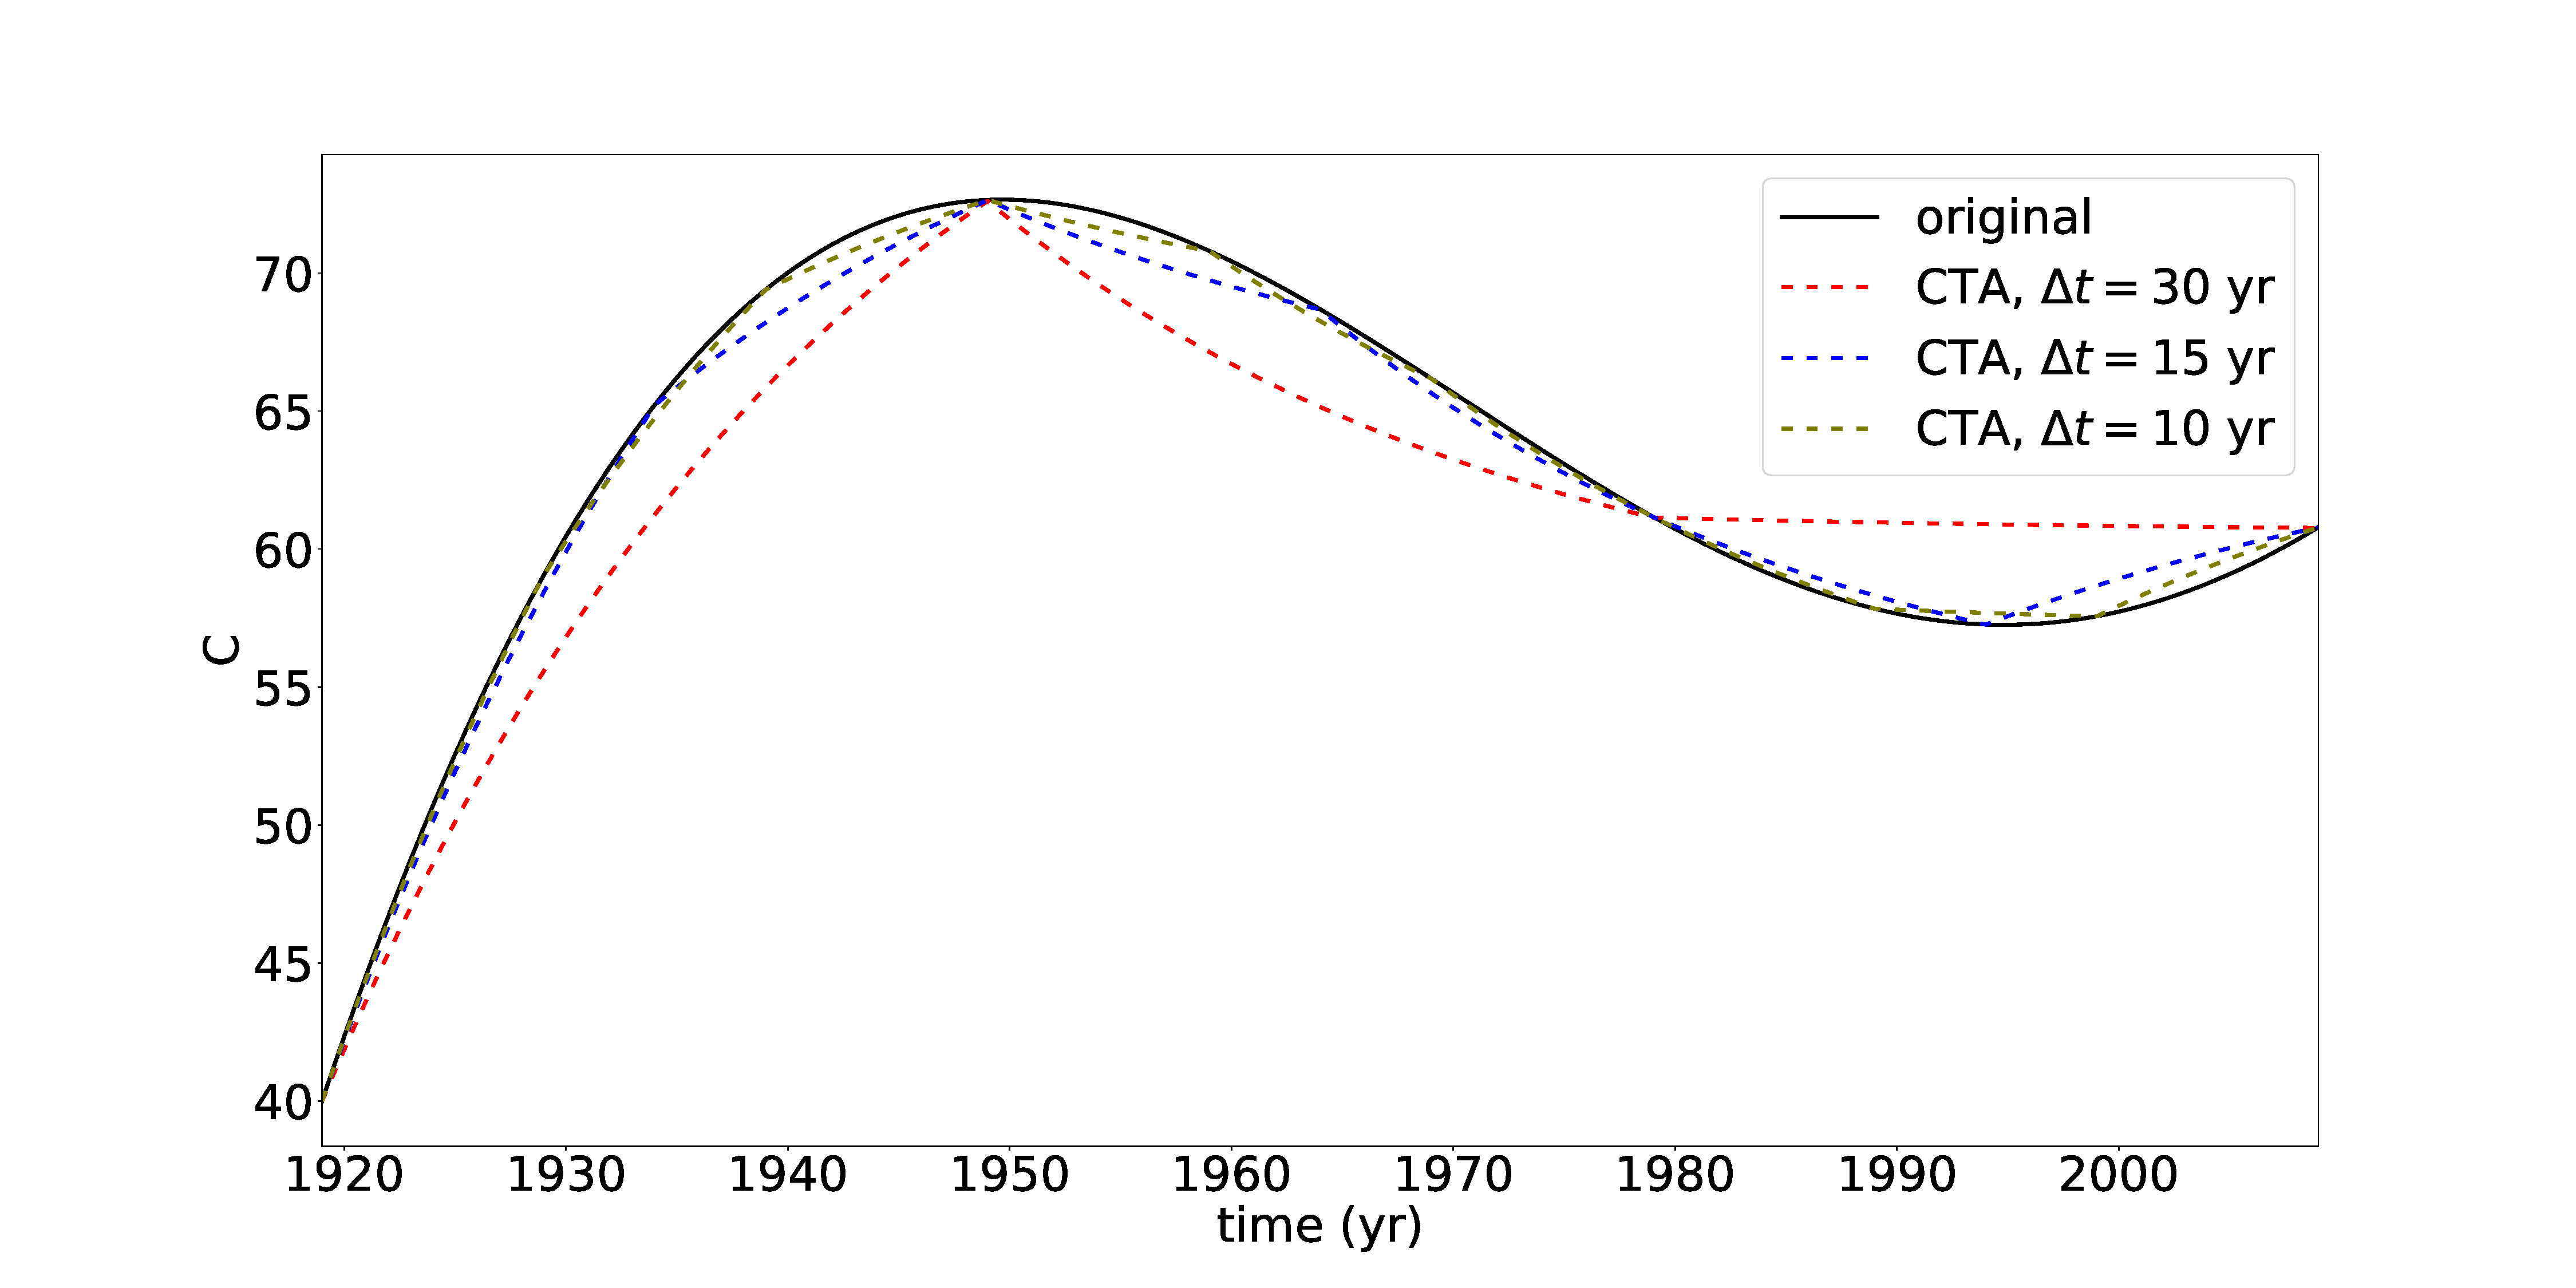
\includegraphics[width=1.0\linewidth]{figs/interpol_pwc_1.pdf}
%    \caption{For the one-compartment system, transient C stocks are well approximated by 10-year time steps. Mean annual absolute bias is X, Y, and Z\% for $\Delta{t}$ = 30, 20, and 10 years, respectively.
%        The solid black line represents the carbon content of the original system \eqref{eqn:CS_one_dim_example}, the dashed red line represents the carbon content of the approximating system.
%        Different panels represent a different number of given equidistant data points, represented by vertical lines.
%        }
    \caption{Quality of transient C stocks of the one-compartment system by CTA for different data time steps $\Delta t$.
    Mean annual absolute bias is $\SI{3.92}{\percent}$, $\SI{0.92}{\percent}$, and $\SI{0.46}{\percent}$ for $\Delta{t} = \SI{30}{\yr}$, $\SI{20}{\yr}$, and $\SI{10}{\yr}$, respectively.
    The solid black line represents the carbon content of the original system \eqref{eqn:CS_one_dim_example}, the dashed lines represent the carbon contents of the CTAs with different time steps.
    }    
    \label{fig:CS_one_dim_example}
\end{figure}        

If we remove the time-dependency from the input boundary condition, the system becomes
%Consider the one-dimensional compartmental system
\begin{equation}\label{eqn:CS_one_dim_example_auton}
    \begin{aligned}
        \deriv{t}\,C(t) &= -0.04\,C(t) + 3,\quad t>1909,\\
        C(1909) &= 40.
    \end{aligned}
\end{equation}
The CTA approach exactly matches the system analytical solution for $n=3,6$ (Figure \ref{fig:CS_one_dim_example_auton}).

\begin{figure}[htbp]
    \centering 
    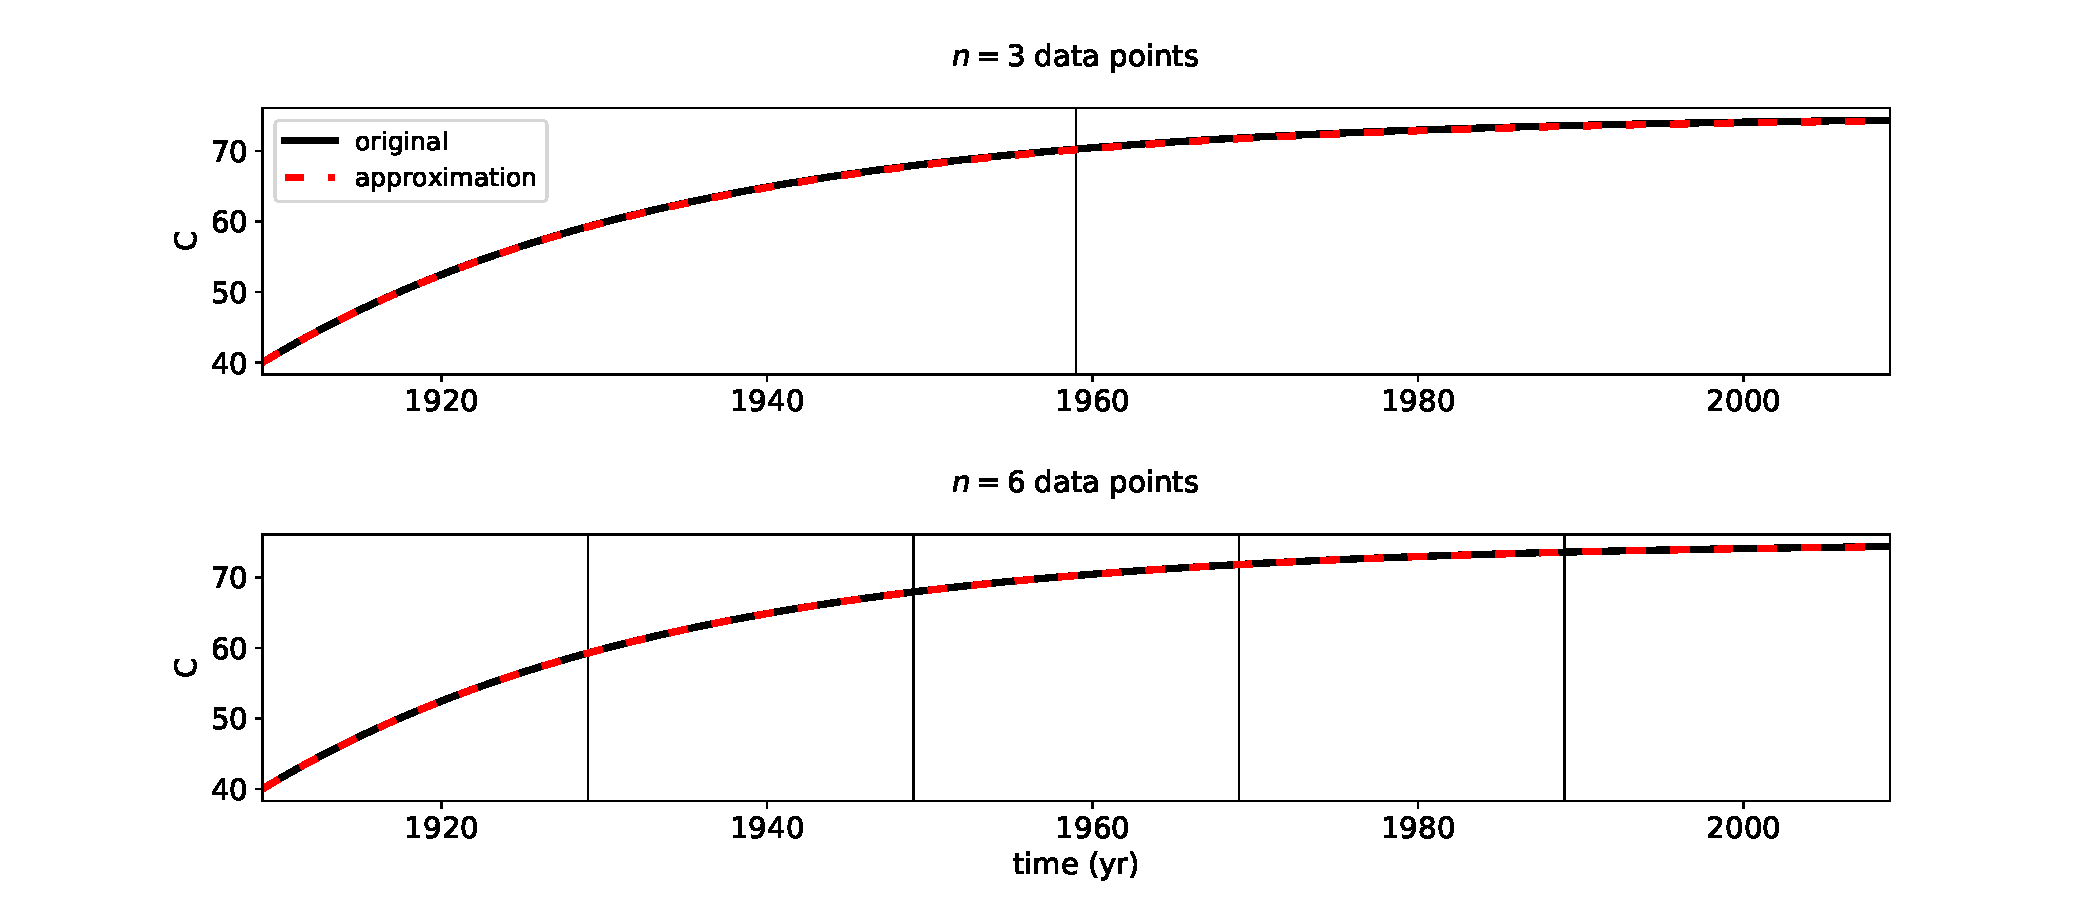
\includegraphics[width=1.0\linewidth]{figs/interpol_pwc_1_auton.pdf}
    \caption{C stocks over time.
        The solid black line represents the carbon content of the original system \eqref{eqn:CS_one_dim_example_auton}, the dashed red line represents the carbon content of the CTA system.
        Different panels represent a different number of given equidistant data points, represented by vertical lines.
        }
    \label{fig:CS_one_dim_example_auton}
\end{figure}        

\subsection{Multi-compartment test}
    As a preliminary test before demonstrating the CTA for the full ELMv1-ECA model reconstruction, we evaluated the approach for several configurations of multiple C pools and non-linear time dependency. We found that the accuracy of the CTA approach does not depend on the number of pools or the non-linear time dependencies. The time step required for accurate reconstruction depends on the frequency of the forcing and non-linear interactions between pools. For example, consider the two compartment system, initialized at $t=1909$, and propagated for 110 years:
    \begin{equation}\label{eqn:CS_two_dim_example}
        \begingroup\makeatletter\def\f@size{10}\check@mathfonts
        \begin{aligned}
            \deriv{t}\,\begin{pmatrix} C_1 \\ C_2 \end{pmatrix}(t) &= 
            \begin{pmatrix} -\gamma_1 & 0.5\,\gamma_2 \\ \gamma_1 & -\gamma_2 \end{pmatrix}(t)\,
            \begin{pmatrix} C_1 \\ C_2 \end{pmatrix}(t) + 
            \begin{pmatrix} 0.5 \\ 0.5 + 0.5\,\sin(t/100) \end{pmatrix}(t),\\
            \begin{pmatrix} C_1 \\ C_2 \end{pmatrix}(1909) &=
            \begin{pmatrix} 40 \\ 0 \end{pmatrix},
        \end{aligned}
        \endgroup
    \end{equation}
    where $\gamma_1(t)=0.1+0.05\,\sin(0.1\,t)$, $\gamma_2(t)=0.05$.
    \todo{this figure can all be collapsed into one panel}
     In this case, data from the original model extracted at 5 y time steps leads to a very accurate CTA (mean absolute error $<$ X\%; Figure \ref{fig:CS_two_dim_example}).
    \begin{figure}[htbp]
        \centering 
        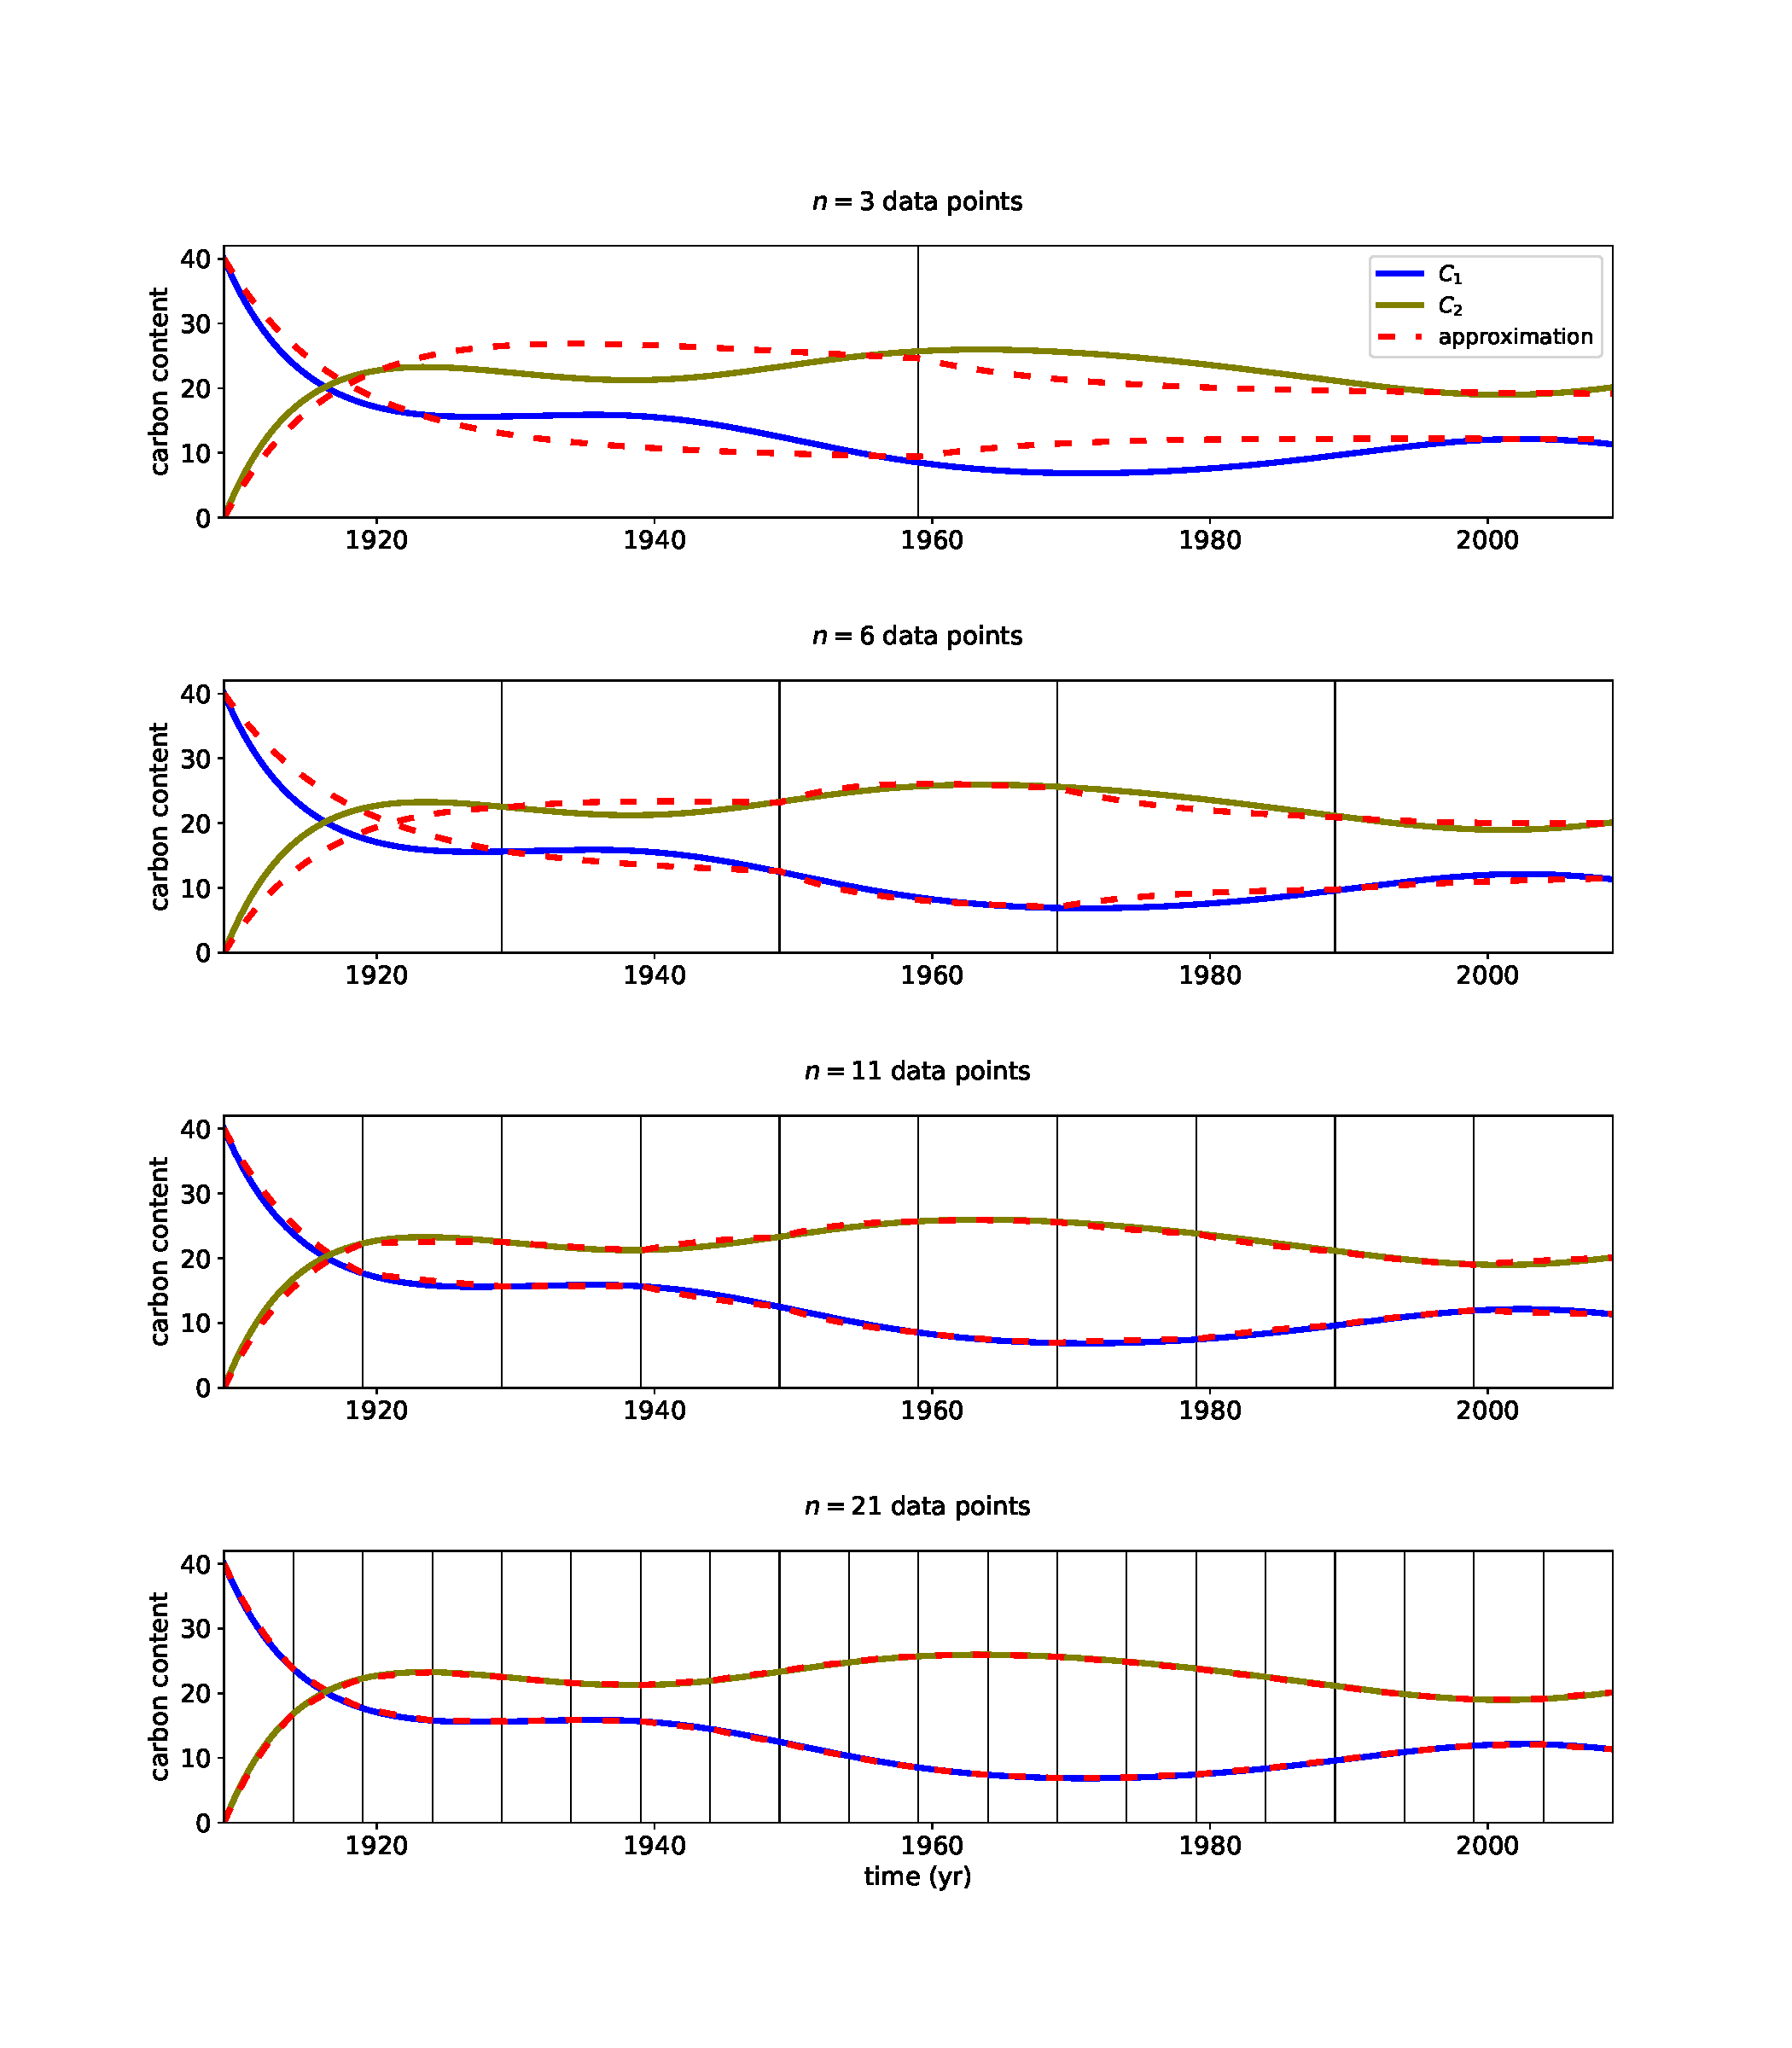
\includegraphics[width=1.0\linewidth]{figs/interpol_pwc_2.pdf}
        \caption{C stocks over time.
            The solid blue and olive curves represent the carbon contents of the two compartments of the original system \eqref{eqn:CS_two_dim_example}, the dashed red lines represent the respective CTAs.
            Different panels represent different numbers of given equidistant data points, represented by vertical lines.
            }
        \label{fig:CS_two_dim_example}
    \end{figure}        

\subsection{ELM Results}

\todo{we need to explain the CTA versus DTA results: why it's slower, just as accurate, etc. Those are Results to report here}

\begin{figure}[htbp]
        \centering 
        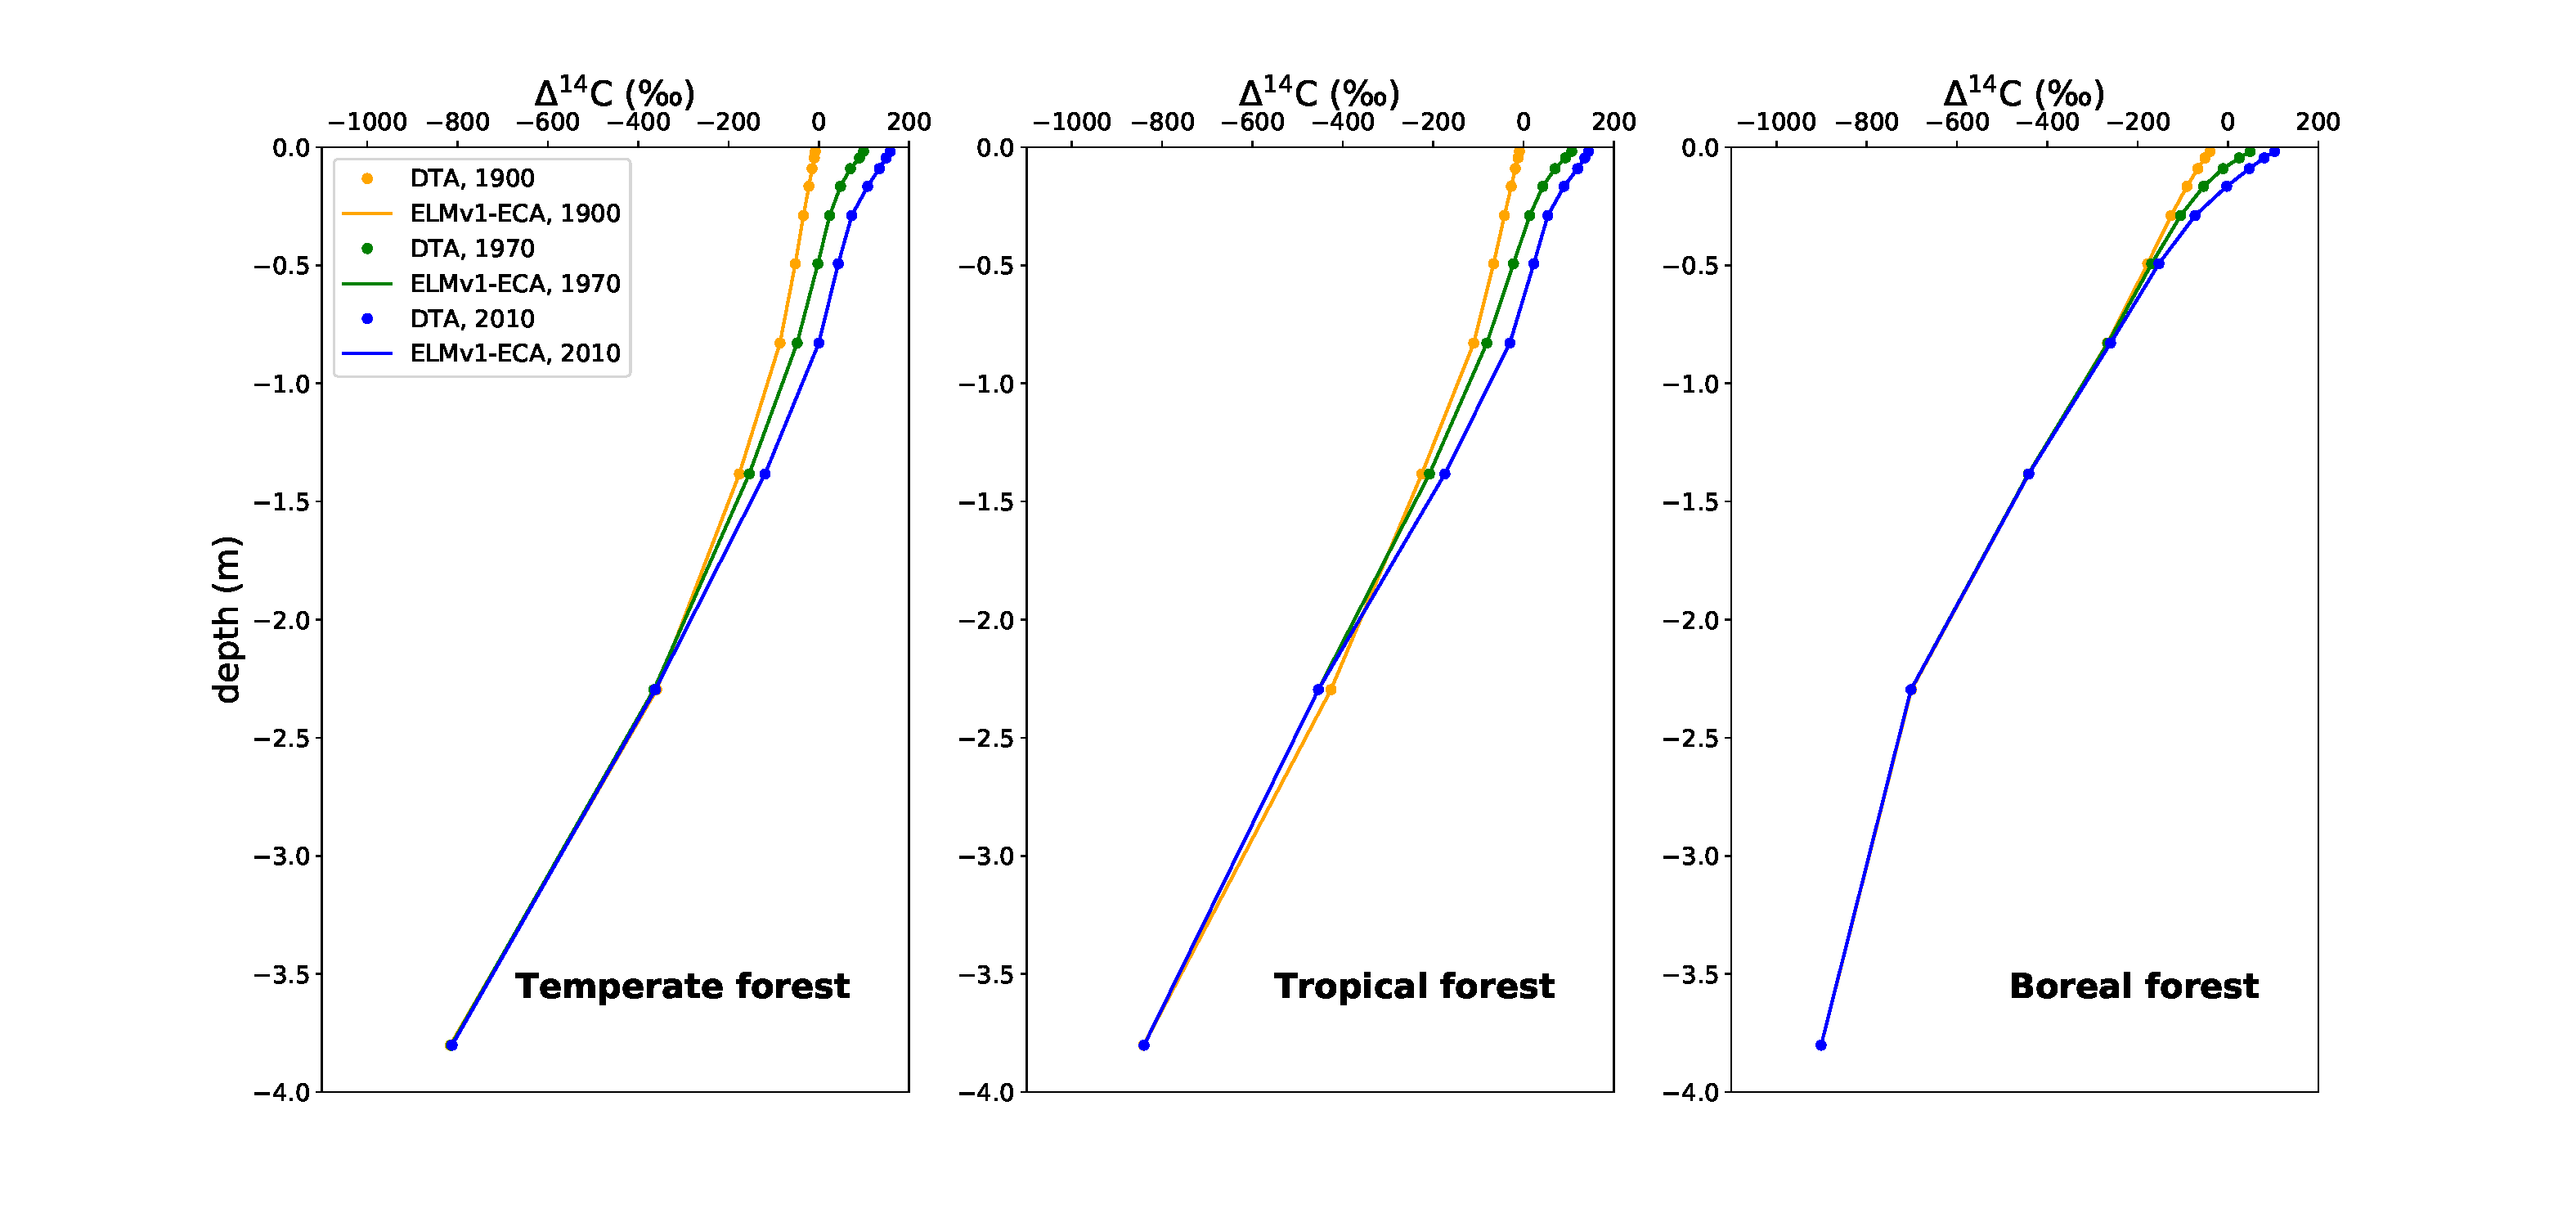
\includegraphics[width=1.0\linewidth]{figs/depth_profile_10.pdf}
        \caption{CTA and ELMv1-ECA modeled $\Delta^{14}$C values with depth in 1900, 1970, and 2010. The CTA bias is less than X\%. Sites (left to right): Boreal, Temperate, Tropical. $\Delta^{14}$C values decrease with depth, and become more enriched following the atmospheric bomb.
            }
            \todo{use "ELMv1-ECA" in legend for consistency. Increase all font sizes by at least a factor of 2. Put site names in lower right of each panel} 
        \label{fig:depthProfiles}
    \end{figure}      

%- demonstration of approach working for different time steps (1 vs 10 d) for ${}^{12}$C (Figure C12_through_time_rel_error_01, *_10.pdf)
%-     same for 14C (Figure C14_through_time_rel_error_01, *_10.pdf)
%- Figure Delta_14C_through_time_per_pools_10.pdf
%- vertical structure (Figure depth_profile_10.pdf; 1 d looks the same)
%- lumping SOC pools by layer, and lumping those lumped SOC by depth interval (e.g., 0-30 cm): this approach doesn't work (i.e., lumping fluxes into a layer, with a lumped single pool in each layer). The lumped single pool cannot represent the internal dynamics.

Using 1-day model output, CTAs of bulk soil $\Delta^{14}$C values accurately reproduced the ELMv1-ECA values for the three sites and for all soil depths (Figure \ref{fig:depthProfiles}). The modeled and CTAs are imperceptibly different across depth for all three sites, with a mean absolute bias of \red{X\%}. 

The CTA also accurately reproduced ELMv1-ECA modeled $\Delta^{14}$C values for all seven pools (coarse woody debris, three litter pools, and three soil pools) over the 110 y simulation (Fig. \ref{fig:poolsOverTime}). For all sites, the mean absolute error is $<0.001$\% for both carbon stocks and $\Delta^{14}$C values across all sites and depths. These extremely low error rates are well within model uncertainty and far less than the observed spatial heterogeneity of soil carbon stocks and radiocarbon values. 
In the 1960s, the radiocarbon concentration in the atmosphere increased sharply due to weapons testing (aka the bomb spike). The CWD, litter, and soil\_1 pools respond relatively rapidly to this change, as atmospheric C is rapidly cycled through these pools. This bomb carbon incorporation into bulk soil is also evident in the top meter of soil (Figure \ref{fig:depthProfiles}). In contrast, the slower soil pools (SOIL\_2, SOIL\_3) have a more lagged and damped response to the atmospheric bomb radiocarbon perturbation.

\begin{figure}[htbp]
        \centering 
        \vspace{-8em}
        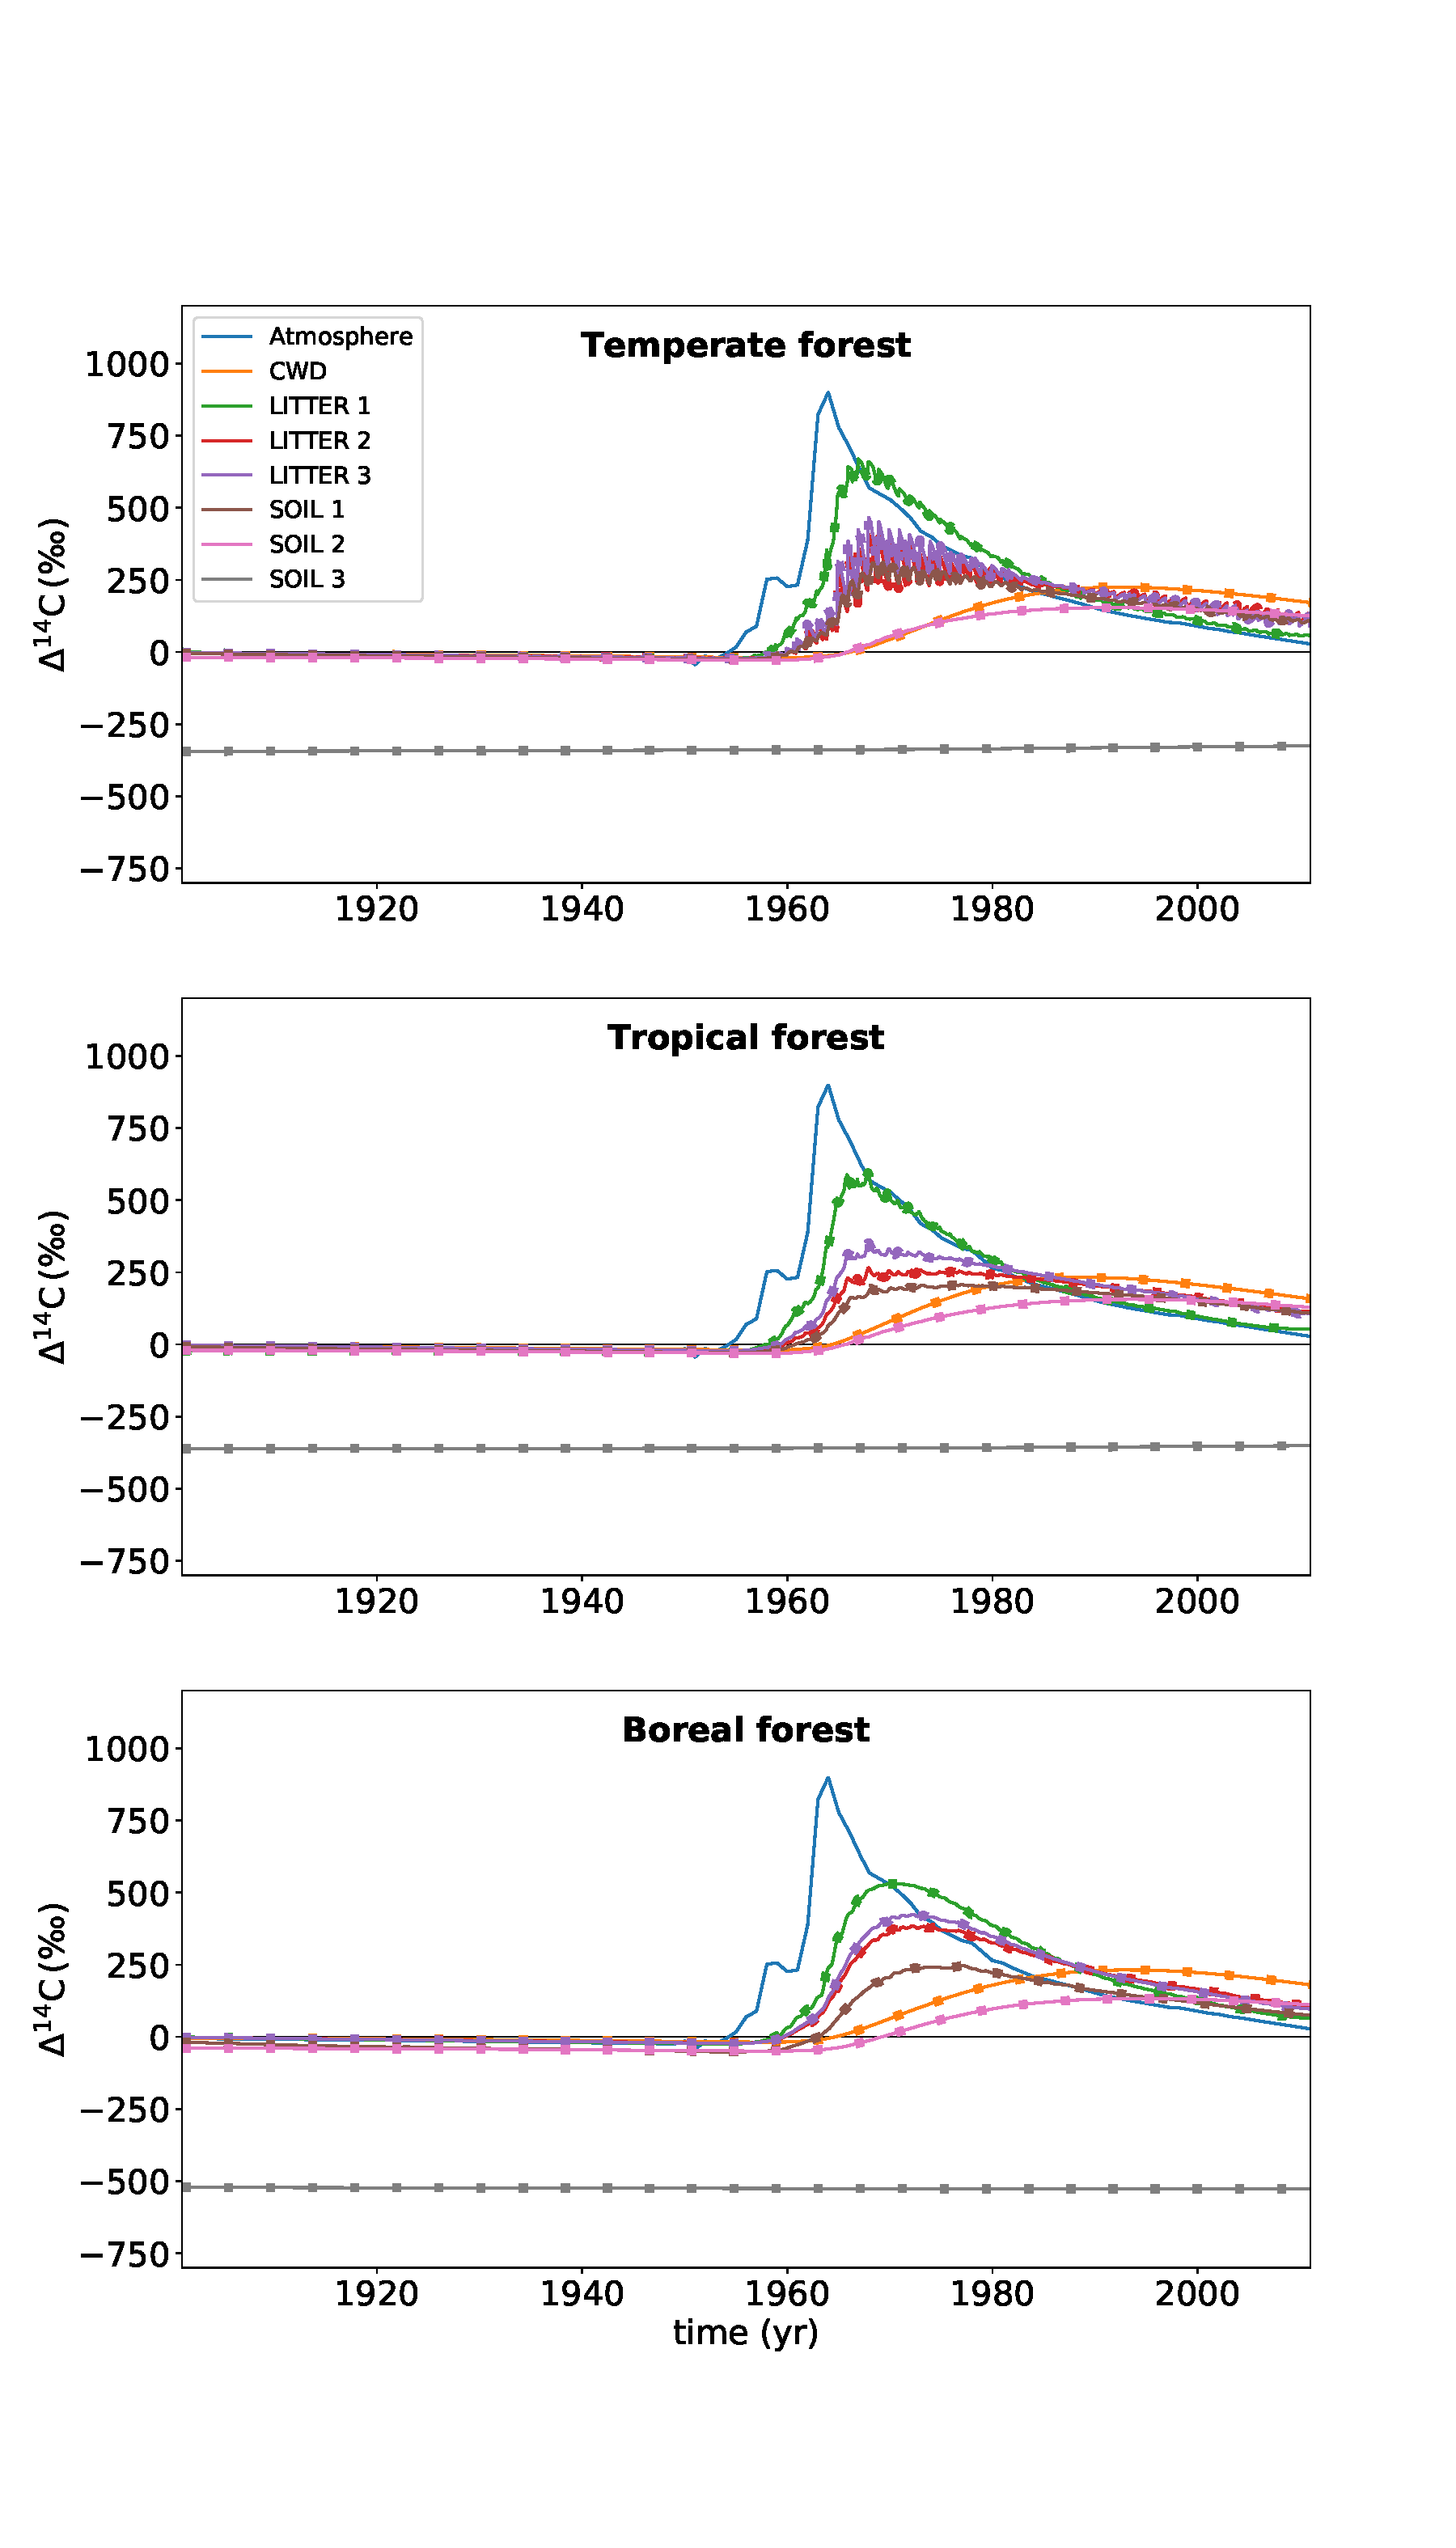
\includegraphics[width=1.0\linewidth]{figs/Delta_14C_through_time_per_pools_10.pdf}
        \vspace{-4em}
        \caption{$\Delta^{14}$C values in all pools through time (Lines: ELMv1-ECA; dots: CTA). Sites (top to bottom): Boreal, Temperate, Tropical. Atmospheric $\Delta^{14}$C values (blue) increase in response to bomb testing in the 1960s. Fast cycling pools increase most rapidly to the atmospheric $\Delta^{14}$C changes. Slower cycling pools show a lagged and damped response. Differences in CTA and ELMv1-ECA modeled values are imperceptible on this figure.
            }
            \todo{put site names inside axis box, increase font by two times for all text in ALL figures. Use permil symbol (or $^o/_{oo}$) on y-axes}
        \label{fig:poolsOverTime}
    \end{figure}    
    
    % Is this figure showing both the computed values and the ELM values on top of each other? Or only the computed values. It is unclear from the legend ...although we know they would look the same, this should be clarified in the legend
    

Although the error rates are extremely low across all pools over time, they vary systematically. The absolute percent error is larger for the CWD and litter pools than for the soil pools, and peaks during the atmospheric bomb period at around 0.025\% \todo{show only Temperate site, make points (1) that largest biases is in litter immediately following the bomb spike and (2) biases are always small} (Fig \ref{fig:10dayErrorOverTime}). The mean absolute percent errors for CTA $\Delta^{14}$C values are in most cases at least two orders of magnitude larger than those for $^{12}$C across sites and pools (Table \ref{tab:ErrorRatios}). The CTA error increases for larger time steps, being an order of magnitude larger for CWD and litter pools in the 10-day versus 1-day time step cases. However, the mean absolute percent error for the 10-day time step case remains very low: $< 1 \times 10^{-5}\,\%$ for $^{12}$C in all pools and sites, and $<0.01\,\%$ for $\Delta^{14}$C in all pools and sites (Table \ref{tab:ErrorRatios}), remaining well within model uncertainty bounds and soil heterogeneity.

\begin{figure}[htbp]
        \centering 
        \vspace{-8em}
        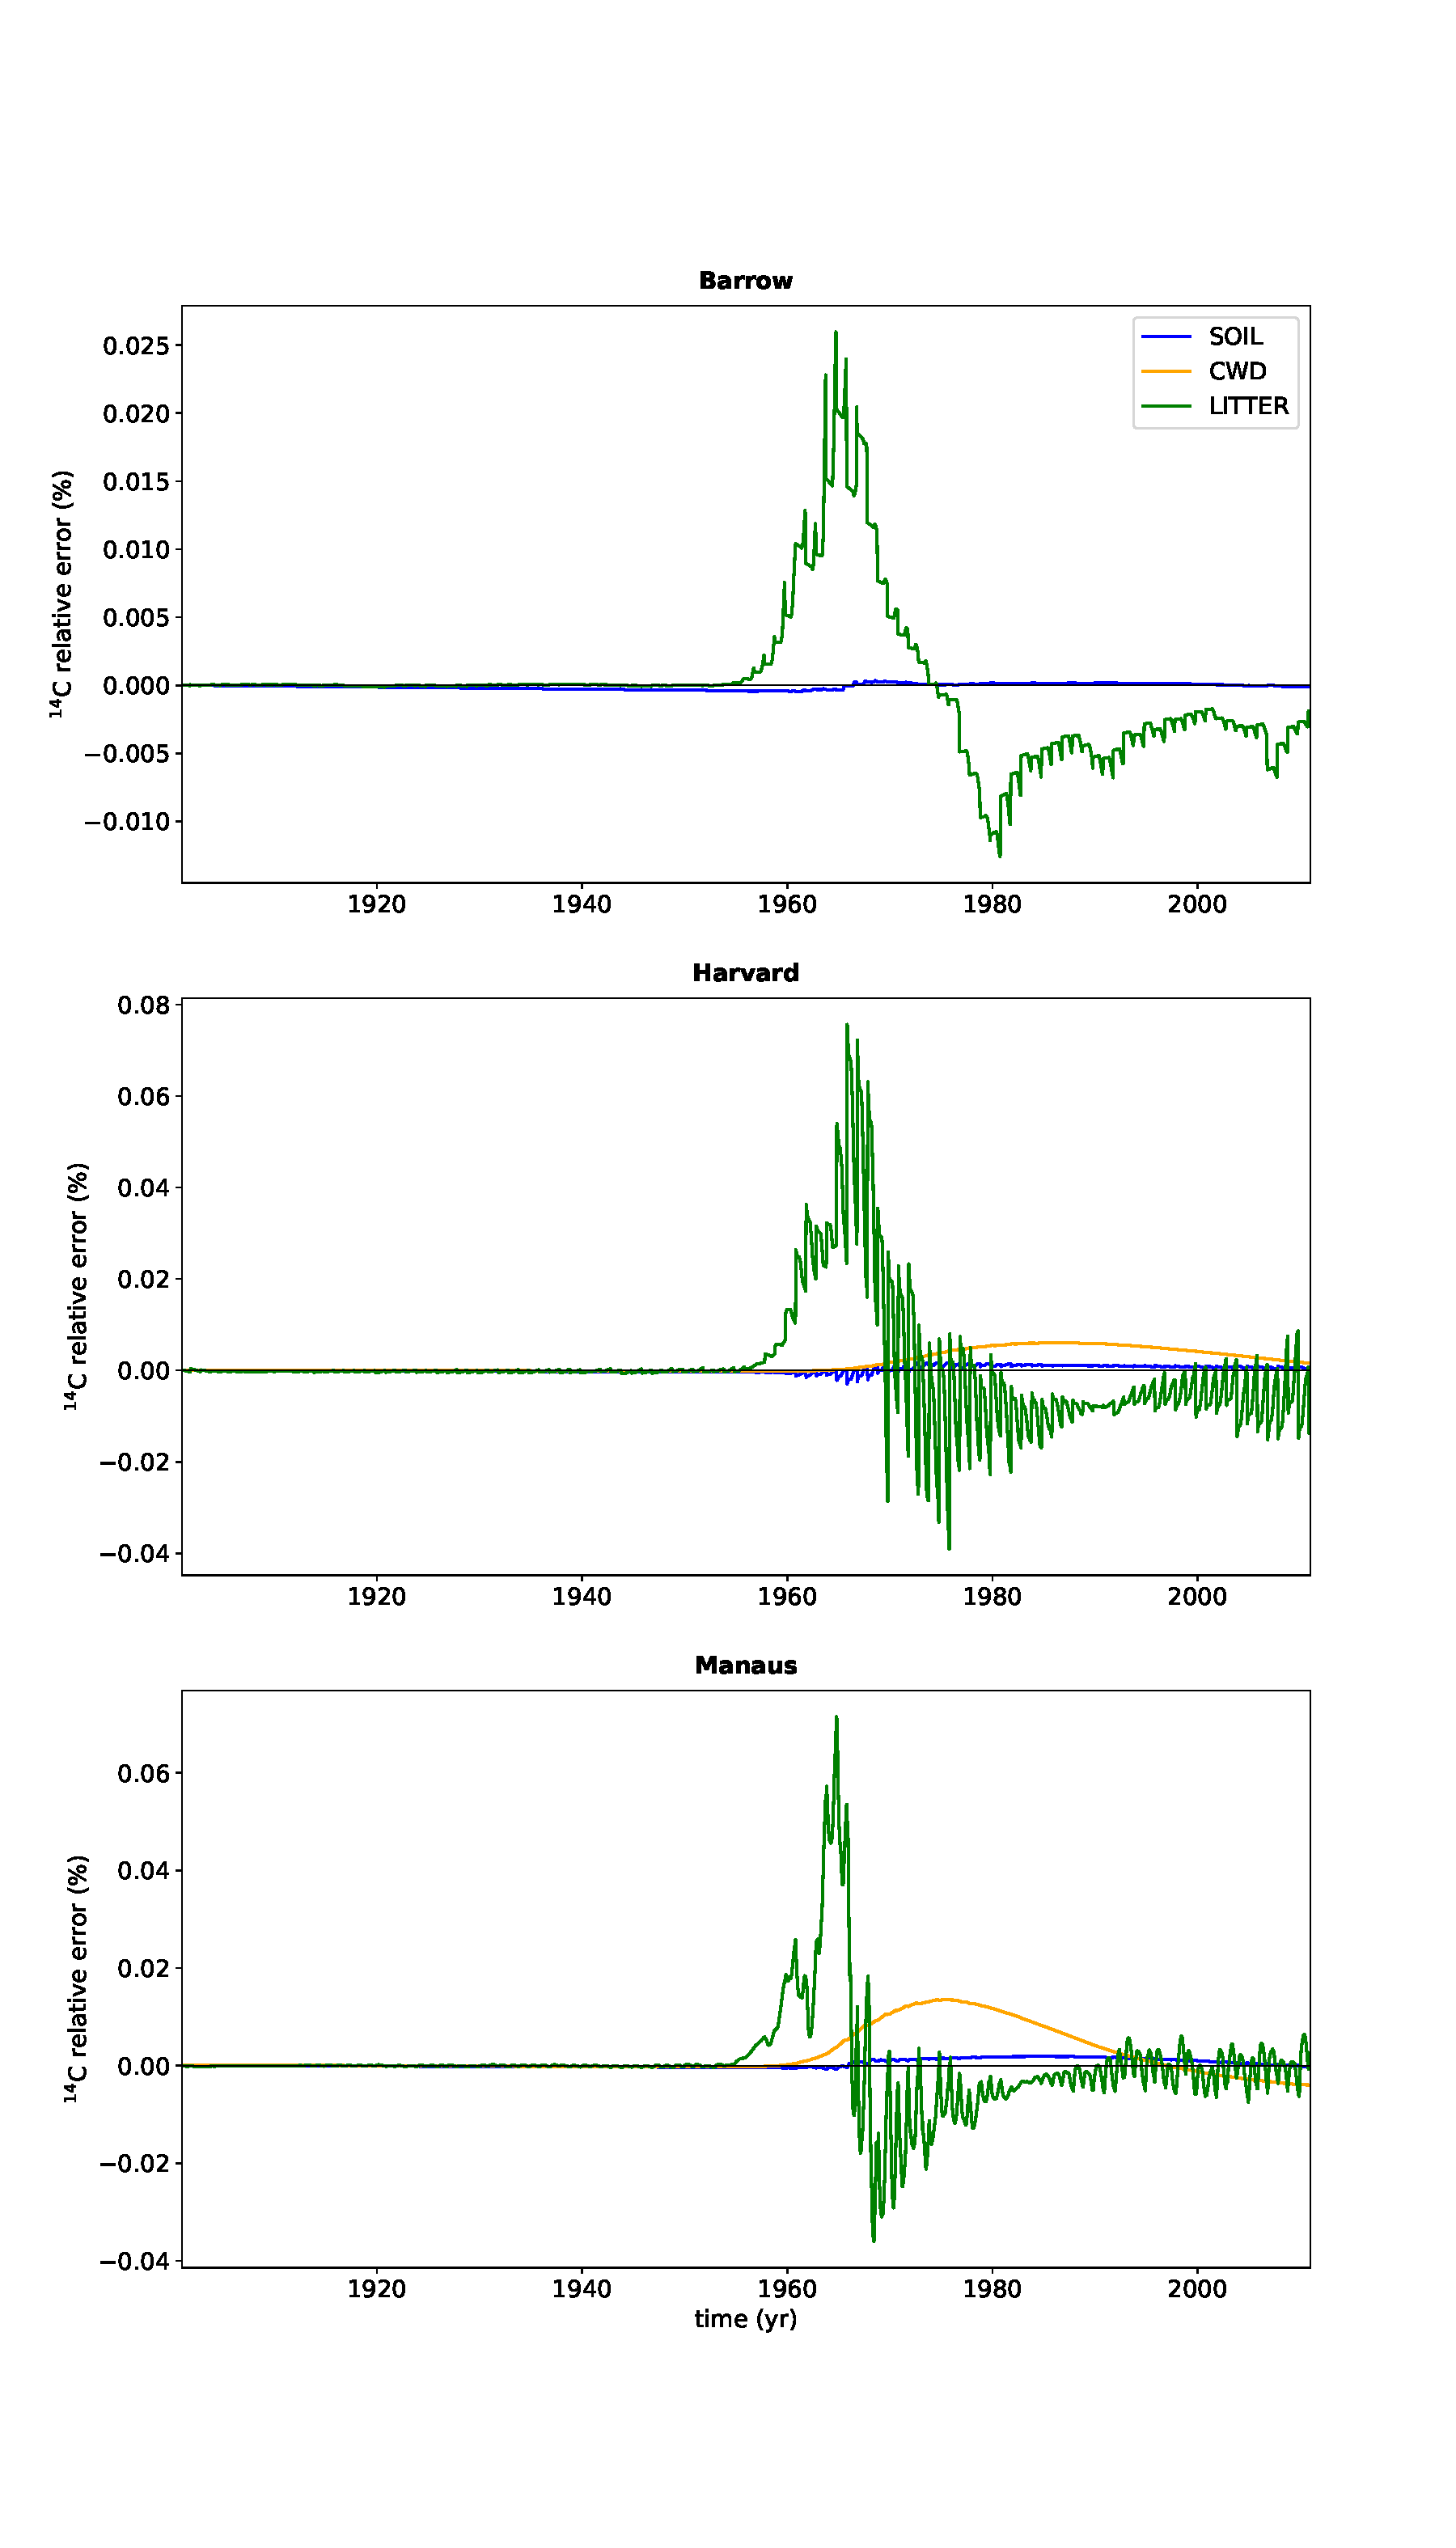
\includegraphics[width=1.0\linewidth]{figs/C14_through_time_rel_err_10.pdf}
        \vspace{-4em}
        \caption{Relative error in radiocarbon values for CWD, litter and soil pools over time. Sites (top to bottom): Boreal, Temperate, Tropical. $^{14}$C percent error is approximately two orders of magnitude larger than $^{12}$C error. 
            }
        \label{fig:10dayErrorOverTime}
\end{figure}    

\begin{sidewaystable}
%\begin{table}[htbp]
\caption{Error ratios of a 10-day and a 1-day timestep reconstruction of ELMv1-ECA.}
\begin{tabular}{lrrrp{0.2cm}lrrrp{0.2cm}lrrr}
\multicolumn{4}{l}{\textbf{10 Day Timestep:}}  &  & \multicolumn{4}{l}{\textbf{1 Day Timestep:}} &  & \multicolumn{4}{l}{\textbf{Ratio of 10-day to 1-day errors}} \\ 
${}^{12}$\textbf{C} &  & &  &  & ${}^{12}$\textbf{C} &  & & &  & ${}^{12}$\textbf{C} &  &  &  \\ 
 & \multicolumn{1}{c}{CWD} & \multicolumn{1}{c}{Litter} & \multicolumn{1}{c}{SOIL} &  &  & \multicolumn{1}{c}{CWD} & \multicolumn{1}{c}{Litter} & \multicolumn{1}{c}{SOIL} &  &  & \multicolumn{1}{c}{CWD} & \multicolumn{1}{c}{Litter} & \multicolumn{1}{c}{SOIL} \\ 
Boreal & - & \num{1.03e-05} & \num{1.50e-06} &  & Boreal & - & \num{1.02E-05} & \num{1.49e-06} &  & Boreal &  & \num{1.0} & \num{1.0} \\ 
Temperate & \num{1.06e-06} & \num{7.52e-06} & \num{1.30e-06} &  & Temperate & \num{1.06e-06} & \num{7.52e-06} & \num{1.29e-06} &  & Temperate & \num{1.0} & \num{1.0} & \num{1.0} \\ 
Tropical & \num{1.04e-06} & \num{3.78e-06} & \num{1.03e-06} &  & Tropical & \num{1.03e-06} & \num{3.76e-06} & \num{1.06e-06} &  & Tropical & \num{1.0} & \num{1.0} & \num{1.0} \\ 
\\ 
${}^{14}$\textbf{C} &  & & &  & ${}^{14}$\textbf{C} &  & & &  & ${}^{14}$\textbf{C}  \\ 
Boreal & - & \num{2.78e-03} & \num{1.81e-04} &  & Boreal & - & \num{3.32e-04} & \num{3.88e-04} &  & Boreal &  & \num{8.4} & \num{0.5} \\ 
Temperate & \num{1.71e-03} & \num{6.22e-03} & \num{5.05e-04} &  & Temperate & \num{1.69e-04} & \num{6.57e-04} & \num{3.01e-04} &  & Temperate & \num{10.1} & \num{9.5} & \num{1.7} \\ 
Tropical & \num{2.79e-03} & \num{4.30e-03} & \num{6.17e-04} &  & Tropical & \num{2.96e-04} & \num{4.77e-04} & \num{2.73e-04} &  & Tropical & \num{9.4} & \num{9.0} & \num{2.3} \\ 
\\ 
\multicolumn{4}{l}{\textbf{Ratio of ${}^{14}$C error to ${}^{12}$C error}} &  & \multicolumn{4}{l}{\textbf{Ratio of ${}^{14}$C error to ${}^{12}$C error}} \\
Boreal & - & \num{270} & \num{121} &  & Boreal &  & \num{33} & \num{261} \\
Temperate & \num{1615} & \num{827} & \num{388} &  & Temperate & \num{160} & \num{87} & \num{233}\\
Tropical & \num{2686} & \num{1138} & \num{599} &  & Tropical & \num{288} & \num{127} & \num{258}\\
\end{tabular}
\label{tab:ErrorRatios}
%\end{table}
\end{sidewaystable}


\section{Discussion}

\subsection{Performance and future application}
The CTA and DTA approaches can be applied to both single-depth and vertically-resolved soil radiocarbon models run at different spatial and temporal resolutions. We recommend using the DTA for reconstructing ESM-scale models, since the CTA computational requirements are much higher. For example, using a 1-day reconstruction of ELMv1-ECA of the period 1860-2010, the CTA computational time was X times higher than using the DTA, and was no more accurate.\todo{Holger: can you evaluate "X"?}

Using a 1-day time step, The DTA very accurately matched ELMv1-ECA modeled $\Delta^{14}$C values ($<$0.001\% relative error). Although the error rate increases for larger time steps, low error ($<$0.01\% relative error) is still achieved at the 10-day time step (Table \ref{tab:ErrorRatios}). These results suggest the error would likely remain within reasonable bounds for a 30-day time step, which is commonly output from most earth system models. 

This CTA approach has widespread applicability, as it can be used across a range of models independent of their underlying structure. The approach does not require models to implement additional isotope dynamics or tracers, but simply to output carbon stocks and fluxes. For maximum accuracy, all model stocks and fluxes are required (e.g., all individual transfers between all pools). Aggregating C stocks results in greatly increased uncertainties. However, given the uncertainties inherent to soil carbon dynamics in Earth System Models, high precision may not be necessary, making partial aggregation a promising line of future research. \todo[color=green!40]{not so sure}

\red{Make sure to cover: (1) what is required to make the approach work (fluxes and states that affect 12C); application to existing models; (2) application to single- and multi-layer models; (3) Discussion on why 12C does better than 14c? Relatedly, why does the soil do so much better than the litter and CWD? }
\subsection{Potential for data-model comparison}

The potential of this approach to add radiocarbon output across a range of models will allow valuable data-model comparisons. This work will enable much more widespread use of radiocarbon as an additional model constraint, particularly in soils. It provides a framework for model intercomparison and will enable the future use of radiocarbon datasets to benchmark and calibrate earth system models.

Although radiocarbon is commonly associated with C age, it cannot be directly interpreted as such in soils, due to mixing of C inputs of different ages in the open system. Instead, radiocarbon measurements and model output are primarily of value as a tracer, and for direct model-data comparison. However, by using a state transition matrix approach, there is the added possibility to calculate ages and transit times from the system \citep{Metzler2018PNAS}. In the future, this approach could be applied to compute radiocarbon values, ages, and transit times across a suite of models. This would allow not only direct data-model validation, but also meaningful conceptual comparisons of the age and transit time of C across model structures. 


\section*{Acknowledgements}
Funding was provided by the Max Planck Society and the German Research Foundation through its Emmy Noether Program (SI 1953/2--1). A.M.H. received funding from the European Research Council (ERC) under the European Union’s Horizon 2020 research and innovation programme (grant agreement No. 695101 (14Constraint)).   

\bibliographystyle{apalike}
%\bibliographystyle{gcb}
\bibliography{refs}


\end{document}